%implementing document formatting:
\documentclass[a4paper,11pt,fleqn,dvipsnames,oneside,openright,oldfontcommands]{memoir} 	% Openright aabner kapitler paa hoejresider (openany begge)


%%%%%%%%% Indsat random
%makes it possible to refer to the name of a chapter rather than just the number.
\usepackage{nameref}
\usepackage{pdfpages}
\usepackage{marvosym}
\usepackage{setspace}
\usepackage{graphicx} % For at sætte 2 billeder ved siden af hinanden

%package for writing program code in latex
\usepackage{listings}
%%%%%%%%%%%%%%%%%%%%%%

% ¤¤ Oversaettelse og tegnsaetning ¤¤ %
\usepackage[T1]{fontenc}					% Output-indkodning af tegnsaet (T1)
\usepackage[danish]{babel}					% Dokumentets sprog
\usepackage[utf8]{inputenc}					% Input-indkodning af tegnsaet (UTF8)
\usepackage{ragged2e,anyfontsize}			% Justering af elementer
\usepackage{fixltx2e}						% Retter forskellige fejl i LaTeX-kernen							
				
																							
% ¤¤ Figurer og tabeller (floats) ¤¤ %
\usepackage{graphicx} 						% Haandtering af eksterne billeder (JPG, PNG, EPS, PDF)
%\usepackage{eso-pic}						% Tilfoej billedekommandoer paa hver side
%\usepackage{wrapfig}						% Indsaettelse af figurer omsvoebt af tekst. \begin{wrapfigure}{Placering}{Stoerrelse}
\usepackage{multirow}                		% Fletning af raekker og kolonner (\multicolumn og \multirow)
\usepackage{multicol}         	        	% Muliggoer output i spalter
\usepackage{rotating}						% Rotation af tekst med \begin{sideways}...\end{sideways}
\usepackage{colortbl} 						% Farver i tabeller (fx \columncolor og \rowcolor)
\usepackage{xcolor}							% Definer farver med \definecolor. Se mere: http://en.wikibooks.org/wiki/LaTeX/Colors
\usepackage{flafter}						% Soerger for at floats ikke optraeder i teksten foer deres reference
\let\newfloat\relax 						% Justering mellem float-pakken og memoir
\usepackage{float}							% Muliggoer eksakt placering af floats, f.eks. \begin{figure}[H]
\usepackage{array,booktabs,xcolor,longtable} % kan lave \hdashline i tabellertabe
\usepackage{arydshln}
\usepackage{tabu}

	
	
% ¤¤ Matematik mm. ¤¤
\usepackage{amsmath , amsthm , amsfonts , amssymb, float, stmaryrd} 		% Avancerede matematik-udvidelser
%\usepackage{mathtools}						% Andre matematik- og tegnudvidelser
\usepackage{textcomp}                 		% Symbol-udvidelser (f.eks. promille-tegn med \textperthousand )
\usepackage{rsphrase}						% Kemi-pakke til RS-saetninger, f.eks. \rsphrase{R1}
\usepackage[version=3]{mhchem} 				% Kemi-pakke til flot og let notation af formler, f.eks. \ce{Fe2O3}
\usepackage{siunitx}						% Flot og konsistent praesentation af tal og enheder med \si{enhed} og \SI{tal}{enhed}
\sisetup{output-decimal-marker = {,}}		% Opsaetning af \SI (DE for komma som decimalseparator) 

% ¤¤ Referencer og kilder ¤¤ %
\usepackage[danish]{varioref}				% Muliggoer bl.a. krydshenvisninger med sidetal (\vref)
\usepackage[numbers]{natbib}				% Udvidelse med naturvidenskabelige citationsmodeller
%\usepackage{xr}							% Referencer til eksternt dokument med \externaldocument{<NAVN>}
%\usepackage{glossaries}					% Terminologi- eller symbolliste (se mere i Daleifs Latex-bog)
\usepackage{lastpage}					% Gør det mulig at refere til sidste side 

% ¤¤ Misc. ¤¤ %
\usepackage{listings}						% Placer kildekode i dokumentet med \begin{lstlisting}...\end{lstlisting}
\usepackage{lipsum}							% Dummy text \lipsum[..]
\usepackage[shortlabels]{enumitem}			% Muliggoer enkelt konfiguration af lister
\usepackage{pdfpages}						% Goer det muligt at inkludere pdf-dokumenter med kommandoen \includepdf[pages={x-y}]{fil.pdf}	
\pdfoptionpdfminorversion=6					% Muliggoer inkludering af pdf dokumenter, af version 1.6 og hoejere
\pretolerance=2500 							% Justering af afstand mellem ord (hoejt tal, mindre orddeling og mere luft mellem ord)


% Kommentarer og rettelser med \fxnote. Med 'final' i stedet for 'draft' udloeser hver note en error i den faerdige rapport.
\usepackage[footnote,draft,danish,silent,nomargin]{fixme}		


%%%% CUSTOM SETTINGS %%%%

% ¤¤ Marginer ¤¤ %
\setlrmarginsandblock{3.0cm}{2.5cm}{*}		% \setlrmarginsandblock{Indbinding}{Kant}{Ratio}
\setulmarginsandblock{2.5cm}{3.0cm}{*}		% \setulmarginsandblock{Top}{Bund}{Ratio}
\checkandfixthelayout 						% Oversaetter vaerdier til brug for andre pakker

%	¤¤ Afsnitsformatering ¤¤ %
\setlength{\parindent}{6mm}           		% Stoerrelse af indryk
\setlength{\parskip}{0mm}          			% Afstand mellem afsnit ved brug af double Enter
\linespread{1,1}							% Linie afstand



% ¤¤ Indholdsfortegnelse ¤¤ %
\setsecnumdepth{subsection}		 			% Dybden af nummerede overkrifter (part/chapter/section/subsection)
\maxsecnumdepth{subsection}					% Dokumentklassens graense for nummereringsdybde
\settocdepth{section} 					% Dybden af indholdsfortegnelsen

% ¤¤ Lister ¤¤ %
\setlist{
  topsep=0pt,								% Vertikal afstand mellem tekst og listen
  itemsep=-1ex,								% Vertikal afstand mellem items
} 

%hyperlinks in the tabel of contents - comment this out before the report is printed.
\usepackage{hyperref}
\hypersetup{
	bookmarks = true,  % Show 'bookmark'-frame in pdf.
	colorlinks = true, % True = colored links, False = framed links.
	citecolor = black,  % Link color for references.
	linkcolor = black,  % Link color in table of contents.
	urlcolor = black,   % Link color for extern URLs.
}

% ¤¤ Opsaetning af figur- og tabeltekst ¤¤ %
\usepackage{caption}
%\usepackage{subcaption}
\captionnamefont{\small\bfseries\itshape}	% Opsaetning af tekstdelen ('Figur' eller 'Tabel')
\captiontitlefont{\small}					% Opsaetning af nummerering
\captiondelim{. }							% Seperator mellem nummerering og figurtekst
\hangcaption								% Venstrejusterer flere-liniers figurtekst under hinanden
%\captionwidth{0.9\textwidth}					% Bredden af figurteksten
\setlength{\belowcaptionskip}{0pt}			% Afstand under figurteksten
\captionsetup[figure]{labelfont={bf,it},font={it}} % sætter nummer til fed og kursis. Resten til fed + skriften er mindre end resten
\captionsetup[table]{labelfont={bf,it},font={it}} 


% ¤¤ Opsaetning af listings ¤¤ %

\definecolor{commentGreen}{RGB}{34,139,24}
\definecolor{stringPurple}{RGB}{208,76,239}

\lstset{language=Matlab,					% Sprog
	basicstyle=\ttfamily\scriptsize,		% Opsaetning af teksten
	keywords={for,if,while,else,elseif,		% Noegleord at fremhaeve
			  end,break,return,case,
			  switch,function},
	keywordstyle=\color{blue},				% Opsaetning af noegleord
	commentstyle=\color{commentGreen},		% Opsaetning af kommentarer
	stringstyle=\color{stringPurple},		% Opsaetning af strenge
	showstringspaces=false,					% Mellemrum i strenge enten vist eller blanke
	numbers=left, numberstyle=\tiny,		% Linjenumre
	extendedchars=true, 					% Tillader specielle karakterer
	columns=flexible,						% Kolonnejustering
	breaklines, breakatwhitespace=true,		% Bryd lange linjer
}

% ¤¤ Navngivning ¤¤ %
\addto\captionsdanish{
	\renewcommand\appendixname{Bilag}
	\renewcommand\contentsname{Indholdsfortegnelse}	
	\renewcommand\appendixpagename{Bilag}
	\renewcommand\appendixtocname{Bilag}
	\renewcommand\cftchaptername{\chaptername~}				% Skriver "Kapitel" foran kapitlerne i indholdsfortegnelsen
	\renewcommand\cftappendixname{\appendixname~}			% Skriver "Appendiks" foran appendiks i indholdsfortegnelsen
}

% ¤¤ Kapiteludssende ¤¤ %
%\definecolor{numbercolor}{gray}{0.7}		% Definerer en farve til brug til kapiteludseende
%\newif\ifchapternonum

\makechapterstyle{AAU}
{
	% Afstand mellem sidehovedet og kapitel+tal+kapitelnavnet defineres til:
	\setlength{\beforechapskip}{0cm}

	% Afstanden mellem kapitelnavnet og body-teksten defineres til:
	\setlength{\afterchapskip}{2cm}

	% Typografiopsætningen til kapitel+tal defineres til:
	\renewcommand\chapnamefont{\sffamily\bfseries\LARGE\raggedright}
	
	% Typografiopsætningen til kapitel+tal defineres til:
	\renewcommand\chaptitlefont{\sffamily\bfseries\huge\color[cmyk]{1.00,0.38,0.00,0.64}}

	% Forårsager, at der til kapitlet også tilføjes dets respektive tal:
	\renewcommand\chapternamenum{}
	\renewcommand\printchapternum
	{
		\makebox[0pt][l]
		{
			\color[cmyk]{1.00,0.38,0.00,0.64}
			\hspace{0.1cm}
			\resizebox{!}{1cm}{\chapnamefont\bfseries\sffamily\thechapter}
		}
	}
	
	% Definitionen af linjenstykket mellem ``Kapitel #'' samt ``kapitelnavnet'':
			\renewcommand\afterchaptertitle{\par\hspace{1.5cm}\hrule height 1pt\vskip\midchapskip}
}

% Aktivering af selve kapitellayoutet med dét navn, som definerer kapitellayoutet (ses fra tidligere):
\chapterstyle{AAU}

%\makechapterstyle{jenor}{					% Definerer kapiteludseende frem til ...
%  \renewcommand\beforechapskip{0pt}
%  \renewcommand\printchaptername{}
%  \renewcommand\printchapternum{}
% % \renewcommand\printchapternonum{\chapternonumtrue}
%  \renewcommand\chaptitlefont{\fontfamily{pbk}\fontseries{db}\fontshape{n}\fontsize{20}{25}\selectfont\raggedright}
%  \renewcommand\chapnumfont{\fontfamily{pbk}\fontseries{m}\fontshape{n}\fontsize{1in}{0in}\selectfont\color{numbercolor}}
% \renewcommand\printchaptertitle[1]{
%    \noindent
%    \ifchapternum
%     \begin{tabularx}{\textwidth}{XI}
%	{\let\\\newline\chaptitlefont ##1\par}     
%    \end{tabularx}
%    \par\vskip-2.5mm\hrule
%    \else
%    \begin{tabularx}{\textwidth}{X}
%      {\parbox[b]{\linewidth}{\chaptitlefont ##1}} & \raisebox{-15pt}{\chapnumfont \thechapter}
%    \end{tabularx}
%    \par\vskip2mm\hrule
%    \fi
%  }
%}											% ... her
%
%\chapterstyle{jenor}						% Valg af kapiteludseende - Google 'memoir chapter styles' for alternativer

% ¤¤ Sidehoved ¤¤ %

\makepagestyle{AAU}							% Definerer sidehoved og sidefod udseende frem til ...
\makepsmarks{AAU}{%
	\createmark{chapter}{left}{shownumber}{}{. \ }
	\createmark{section}{right}{shownumber}{}{. \ }
	\createplainmark{toc}{both}{\contentsname}
	\createplainmark{lof}{both}{\listfigurename}
	\createplainmark{lot}{both}{\listtablename}
	\createplainmark{bib}{both}{\bibname}
	\createplainmark{index}{both}{\indexname}
	\createplainmark{glossary}{both}{\glossaryname}
}
\nouppercaseheads											% Ingen Caps oenskes

\makeoddhead{AAU}{Gruppe 375}{}{\leftmark}				% Definerer lige siders sidehoved (\makeevenhead{Navn}{Venstre}{Center}{Hoejre})
\makeevenhead{AAU}{\rightmark}{}{Aalborg Universitet}		% Definerer ulige siders sidehoved (\makeoddhead{Navn}{Venstre}{Center}{Hoejre})
\makeevenfoot{AAU}{Side \thepage\ af \pageref{LastPage}}{}{}							% Definerer lige siders sidefod (\makeevenfoot{Navn}{Venstre}{Center}{Hoejre})
\makeoddfoot{AAU}{}{}{Side \thepage\ af \pageref{LastPage}}								% Definerer ulige siders sidefod (\makeoddfoot{Navn}{Venstre}{Center}{Hoejre})
\makeheadrule{AAU}{\textwidth}{0.5pt}						% Tilfoejer en streg under sidehovedets indhold
\makefootrule{AAU}{\textwidth}{0.5pt}{1mm}					% Tilfoejer en streg under sidefodens indhold

\copypagestyle{AAUchap}{AAU}								% Sidehoved for kapitelsider defineres som standardsider, men med blank sidehoved
\makeoddhead{AAUchap}{}{}{}
\makeevenhead{AAUchap}{}{}{}
\makeheadrule{AAUchap}{\textwidth}{0pt}
\aliaspagestyle{chapter}{AAUchap}							% Den ny style vaelges til at gaelde for chapters
															% ... her
															
\pagestyle{AAU}												% Valg af sidehoved og sidefod


%%%% CUSTOM COMMANDS %%%%

% ¤¤ Billede hack ¤¤ %
\newcommand{\figur}[4]{
		\begin{figure}[H] \centering
			\includegraphics[width=#1\textwidth]{billeder/#2}
			\caption{#3}\label{#4}
		\end{figure} 
}

% ¤¤ Specielle tegn ¤¤ %
\newcommand{\decC}{^{\circ}\text{C}}
\newcommand{\dec}{^{\circ}}
\newcommand{\m}{\cdot}


%%%% ORDDELING %%%%

\hyphenation{}

%%%%Fra engelsk til dansk i \autoref{•} %%%%
\renewcommand{\figureautorefname}{figur}
\renewcommand{\sectionautorefname}{afsnit}
\renewcommand{\subsectionautorefname}{afsnit}
\renewcommand{\subsubsectionautorefname}{afsnit}
\renewcommand{\tableautorefname}{tabel}
\renewcommand{\appendixautorefname}{bilag}
\renewcommand{\equationautorefname}{ligning}
\renewcommand{\itemautorefname}{punkt}
\renewcommand{\chapterautorefname}{kapitel}
%Figure references:
\newcommand{\figref}[1]{\textbf{figur \ref{#1}}}

%Figure references after full stop/period:
\newcommand{\Figref}[1]{\textbf{Figur \ref{#1}}}

%Table references:
\newcommand{\tableref}[1]{\textbf{tabel \ref{#1}}}

%Table references after full stop/period:
\newcommand{\Tableref}[1]{\textbf{Tabel \ref{#1}}}

%Units:
%inserting '\omit' before '{\put' prior ot final compile will fix allignment (and generate errors)
\newcommand{\unit}[1]{{\put(300,0){$\hfill\left[\: #1 \:\right]$}}}

%Text:
\newcommand{\tx}[1]{\text{#1}}

%Equation references:
%1 equation:
\renewcommand{\eqref}[1]{\textbf{ligning (\ref{#1})}}
%2 equations:
\newcommand{\eqrefTwo}[2]{\textbf{ligning (\ref{#1})} and \textbf{(\ref{#2})}}
%3 equations:
\newcommand{\eqrefThree}[3]{\textbf{ligning (\ref{#1})}, \textbf{(\ref{#2})} and \textbf{(\ref{#3})}}
%4 equations:
\newcommand{\eqrefFour}[4]{\textbf{ligning (\ref{#1})}, \textbf{(\ref{#2})}, \textbf{(\ref{#3})} and \textbf{(\ref{#4})}}
%5 equations:
\newcommand{\eqrefFive}[5]{\textbf{ligning (\ref{#1})}, \textbf{(\ref{#2})}, \textbf{(\ref{#3})}, \textbf{(\ref{#4})} and \textbf{(\ref{#5})}}
%5 equations:
\newcommand{\eqrefSix}[6]{\textbf{ligning (\ref{#1})}, \textbf{(\ref{#2})}, \textbf{(\ref{#3})}, \textbf{(\ref{#4})}, \textbf{(\ref{#5})} and \textbf{(\ref{#6})}}
%5 equations:
\newcommand{\eqrefSeven}[7]{\textbf{ligning (\ref{#1})}, \textbf{(\ref{#2})}, \textbf{(\ref{#3})}, \textbf{(\ref{#4})}, \textbf{(\ref{#5})}, \textbf{(\ref{#6})} and \textbf{(\ref{#7})}}

%Equation references after full stop/period:
%1 equation:
\newcommand{\Eqref}[1]{\textbf{Ligning (\ref{#1})}}
%2 equations:
\newcommand{\EqrefTwo}[2]{\textbf{Ligning (\ref{#1})} and \textbf{(\ref{#2})}}
%3 equations:
\newcommand{\EqrefThree}[3]{\textbf{Ligning (\ref{#1})}, \textbf{(\ref{#2})} and \textbf{(\ref{#3})}}
%4 equations:
\newcommand{\EqrefFour}[4]{\textbf{Ligning (\ref{#1})}, \textbf{(\ref{#2})}, \textbf{(\ref{#3})} and \textbf{(\ref{#4})}}
%5 equations:
\newcommand{\EqrefFive}[5]{\textbf{Ligning (\ref{#1})}, \textbf{(\ref{#2})}, \textbf{(\ref{#3})}, \textbf{(\ref{#4})} and \textbf{(\ref{#5})}}
%5 equations:
\newcommand{\EqrefSix}[6]{\textbf{Ligning (\ref{#1})}, \textbf{(\ref{#2})}, \textbf{(\ref{#3})}, \textbf{(\ref{#4})}, \textbf{(\ref{#5})} and \textbf{(\ref{#6})}}
%5 equations:
\newcommand{\EqrefSeven}[7]{\textbf{Ligning (\ref{#1})}, \textbf{(\ref{#2})}, \textbf{(\ref{#3})}, \textbf{(\ref{#4})}, \textbf{(\ref{#5})}, \textbf{(\ref{#6})} and \textbf{(\ref{#7})}}
\begin{document}

%||||||||||||||||||||||||||||||||||||||||||||||||||||||||||||||||
%|||||||				Example Inputs					 ||||||||
%||||||||||||||||||||||||||||||||||||||||||||||||||||||||||||||||
%|||||||												 ||||||||
%	\section{Figure Sample}

\begin{figure}[H]
	\caption{CAPTION\fxnote{Remember source}}
	\label{LABEL}
	\centering
	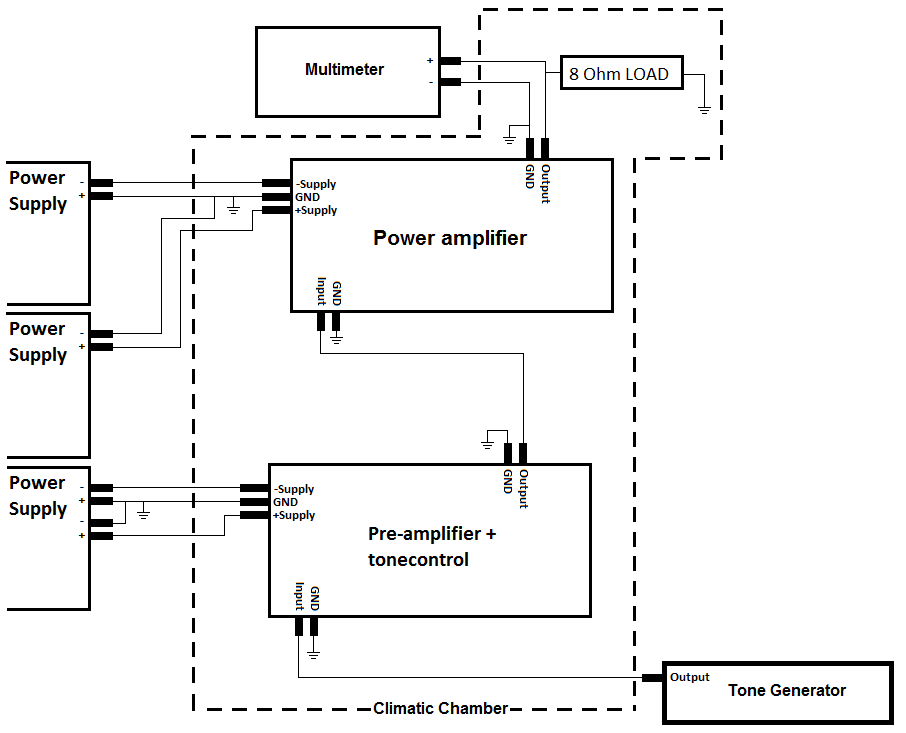
\includegraphics[scale=.8]{figures/filename}
	\flushleft
	\textit{SOURCE}
\end{figure}

%--------- NOTES ------------------------------------------------------
%Fxnotes wont compile properly inside the figure, only in the caption.
%Filetype can be specified but isn't needed.

\noindent
\figref{LABEL}\\

\noindent
\Figref{LABEL}

\vspace{.5cm}
%Do not use \vspace{length} or \hspace{length} unless exceedingly necessary.

%--------- BIBLIOGRAPHY REF EKSAMPLE -----------------------------------
This reference only represents this line since it is before the punctuation mark\cite{YDing}. This next reference however represents the entire section. That is all of the preceding sentences in the entire section. This is due to the fact that it is now after the punctuation mark in the end of the section (this is not used in the middle of a section!).\cite{YDing}
%>>>>>>>>>>>>>>>PLEASE ALSO READ THE NOTE IN myBib.bib<<<<<<<<<<<<<<<<<<
\pagebreak	%||||||||
%	\section{Table Sample}

\begin{table}[H]
\caption{This Is a Table\label{LABEL}}
\begin{tabular}{|l|p{5cm}|l|l|l|}
  \hline
  \textbf{No.}&\textbf{Description}&\textbf{Min}&\textbf{Max}&\textbf{Requirements}\\
  \hline
  1 & Some Text & Some Text & Some Text & Some Text\\
    &           &           &           & Some More Text\\
    &           &           &           & Text Text\\
    &           &           &           & Text Text Text\\
  \hline
  2 & Some Text & Some Text & Some Text & Some Text\\
  \hline
  3 & 	By specifying the width of a column (|p\{5cm\}|) the cells
  		in that column will will not exceed	the specified width    %Enter is used only for clarity and will not affect the compiled output.
  		but instead expand downward.
  		
  		        & Some Text & Some Text & Some Text\\
  \hline
  4 & Some Text & Some Text & Some Text & Some Text\\
  \hline
  \multicolumn{2}{|l|}{Some Text} 	&	\multicolumn{3}{l|}{Some Text}\\
  \hline
  \multicolumn{2}{|l|}{Text Text} 	&	\multicolumn{3}{l|}{Text = Text}\\
  \multicolumn{2}{|l|}{}			&	\multicolumn{3}{l|}{Text = Text}\\
  \multicolumn{2}{|l|}{}			&	\multicolumn{3}{l|}{Text = Text}\\
  \multicolumn{2}{|l|}{}			&	\multicolumn{3}{l|}{Text = Text}\\
  \multicolumn{2}{|l|}{}			&	\multicolumn{3}{l|}{Text = Text}\\
  \hline
  \multicolumn{2}{|l|}{Some Text} 	&	\multicolumn{3}{l|}{Teeeexxtt}\\
  \multicolumn{2}{|l|}{}			&	\multicolumn{3}{l|}{\LaTeX}\\
  \hline      
\end{tabular}
\end{table}

\noindent
\tableref{LABEL}\\

\noindent
\Tableref{LABEL}

\pagebreak	%||||||||
%	\section{Equation Sample}

\noindent
Some explanation:
%
\begin{align}
\unit{Unit}
[Equation]&=[Number]
\label{eq1}
\end{align}

\noindent
Some other explanation:
%
\begin{align}
\unit{Unit}
[Equation]&=[Number]
\label{eq2}
\end{align}

\noindent
Yet an explanation:
%
\begin{align}
\unit{Unit}
\text{You see? } [Equation]&=[Number]
\label{eq3}\\
%
\unit{Unit}
\text{Unit isn't aligned } \textbf{:( } \: [Equation]&=[Number]
\label{eq4}	   %
\end{align}	 	%
			  	 %
\noindent	   	  %
Explanation!:	   %
%				 	%
\begin{align}	  	 %
\unit{Unit}		   	  %
[Equation]&=[Number]   %	%-----------------------NOTES-----------------------%
\label{eq5}\\		 	%	% The &-sign aligns the equal signs.				%
%					  	 %	%													%
\unit{Unit}			   	  % % \unit{} will not be alligned by default,			%
[Equation]&=[Number]	   %% however the macro can be modded as described 		%
\label{eq6}\\			    % in macros.tex. This will allign the units,		%
%						    % but generate errors.								%
\unit{Unit}				    %													%
[Equation]&=[Number]		% \noindent should generally be used befor			%
\label{eq7}					% oneliners after equations, figures and tables.	%
\end{align}					%---------------------------------------------------%
\\
%
\noindent
\eqref{eq1}\\
\noindent
\eqrefTwo{eq1}{eq2}\\
\noindent
\eqrefThree{eq1}{eq2}{eq3}\\
\noindent
\eqrefFour{eq1}{eq2}{eq3}{eq4}\\
\noindent
\eqrefFive{eq1}{eq2}{eq3}{eq4}{eq5}\\
\noindent
\eqrefSix{eq1}{eq2}{eq3}{eq4}{eq5}{eq6}\\
\noindent
\eqrefSeven{eq1}{eq2}{eq3}{eq4}{eq5}{eq6}{eq7}\\
\noindent
\Eqref{eq1}\\
\noindent
\EqrefTwo{eq1}{eq2}\\
\noindent
\EqrefThree{eq1}{eq2}{eq3}\\
\noindent
\EqrefFour{eq1}{eq2}{eq3}{eq4}\\
\noindent
\EqrefFive{eq1}{eq2}{eq3}{eq4}{eq5}\\
\noindent
\EqrefSix{eq1}{eq2}{eq3}{eq4}{eq5}{eq6}\\
\noindent
\EqrefSeven{eq1}{eq2}{eq3}{eq4}{eq5}{eq6}{eq7}
\pagebreak	%||||||||
%|||||||												 ||||||||
%||||||||||||||||||||||||||||||||||||||||||||||||||||||||||||||||
%||||||||||||||||||||||||||||||||||||||||||||||||||||||||||||||||
%\iffalse
%--------------------Introduktion--------------------------------
\chapter{Indledning}\label{Indledning}
% !TeX spellcheck = da_DK
\subsection{Indledning}
heuhkehhorho
\input{rapportAfsnit/bInitierende/initierende_spg}

%-----------------------Problemanalyse---------------------------
\chapter{Problemanalyse}
\section{Amyotrofisk lateral sklerose} \label{sec:ALS}
ALS er en neurodegenerativ sygdom, der påvirker motorneuronerne i hjernen, hjernestammen og rygsøjlen i takt med sygdommens fremskriden, hvilket resulterer i muskelsvaghed \citep{henschke2012}. 
En illustration af, hvordan ALS påvirker motorneuroner, illustreres på \autoref{fig:affectedneuron}. 
De første symptomer på sygdommen er kramper, svaghed samt stive muskler, hvilket kan opstå som muskelsvaghed i arme eller ben, talebesvær eller svaghed i de muskler, som styrer respirationen \citep{nationalinstitute2016}. 
Symptomer og følger af ALS varierer fra patient til patient, hvorved nogle patienter først oplever muskelsvaghed i deres ben, mens andre oplever muskelsvaghed i deres hænder og arme eller besvær ved tale- eller synkebesvær \citep{nationalinstitute2016, miller2005}.

\begin{figure}[H]
\centering
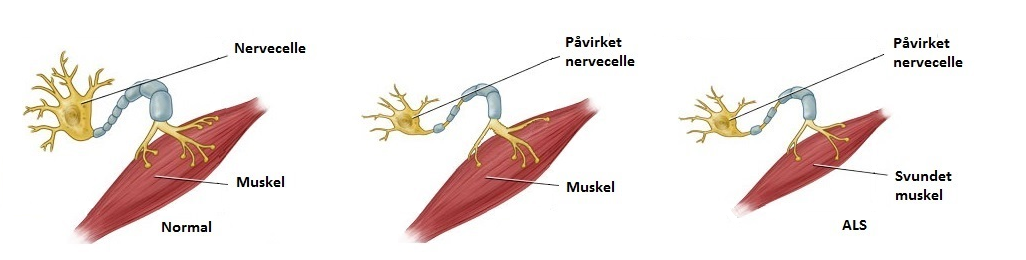
\includegraphics[width=1\textwidth]{figures/affectedneuron}
\caption{Nervecelle og muskel påvirket af ALS. Til venstre ses en normal motorneuron samt en upåvirket muskel. I midten fremgår motorneuronet påvirket af ALS, dog ses musklen endvidere upåvirket. Til højre ses motorneuronet påvirket, samt at musklen er svundet ind. Svindet skyldes en manglende stimulering af musklen som følge af den påvirkede motorneuron \citep{drake2015}.}
\label{fig:affectedneuron}
\end{figure}
 
\noindent
Muskelsvagheden skyldes abnormiteter i de nedre motorneuroner. De nedre motorneuroner er de nerveceller, der videregiver information fra rygmarven til musklerne. 
Symptomer på abnormiteter i de nedre motorneuroner ses som muskelsvaghed samt muskelkramper og atrofi.
Ligeledes kan de øvre motorneuroner påvirkes. Disse motorneuroner sørger for kommunikationen mellem hjernen og de nedre motorneuroner i rygmarven. 
Ved abnormitet, opstår komplikationer ved vidersendelse af beskeder til det givne sted. 
Dette ses som spasticitet samt overdrevne reflekser \citep{nationalinstitute2016}. Opdelingen af de nedre samt øvre motorneuroner ses på \autoref{fig:motorneuroner}.

\begin{figure}[H]
\centering
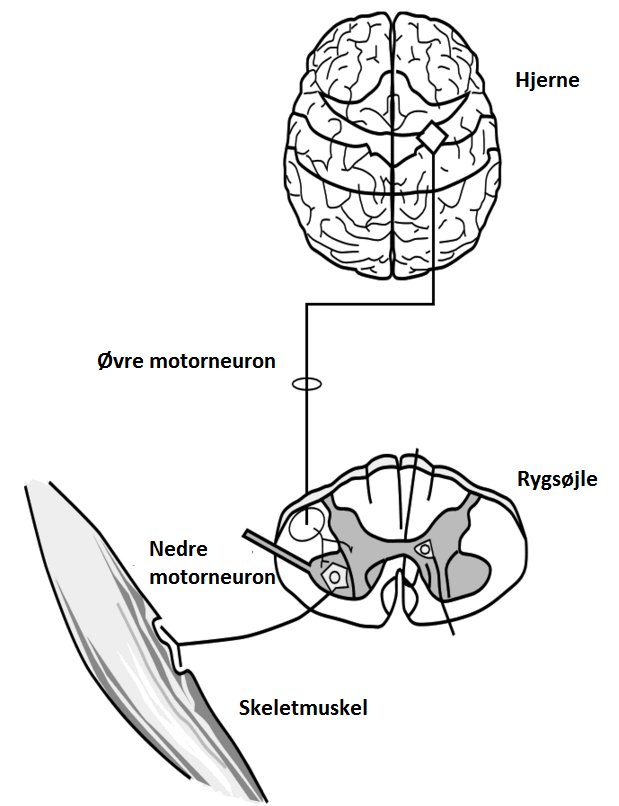
\includegraphics[width=0.6\textwidth]{figures/motorneuroner.png}
\caption{Illustrerer opdelingen af de nedre samt øvre motorneuroner i forhold til hjernen, rygsøjlen og skeletmuskulaturen \citep{miller2005}.}
\label{fig:motorneuroner}
\end{figure}

\noindent
Årsagen til ALS' opståen er oftest ukendt, dog ses en arvelighed i $5 - 10~\%$ af tilfældene. Heraf anslås, at $20~\%$ har det muterede Superocide dismutase 1-gen (SOD-1), hvilket resulterer i tab af motorneuroner \citep{miller2005}.

På trods af, at ALS opleves individuelt både i forhold til sygdomsprogressionen samt, hvilke komplikationer de oplever, kan sygdommen inddeles i tre stadier: et tidligt, midt og endeligt stadie. Et diagram af de tre stadier fremgår af \autoref{fig:stadier}.

\begin{figure}[H]
\centering
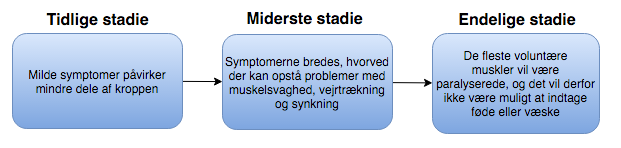
\includegraphics[width=1\textwidth]{figures/stadier.png}
\caption{Tre stadier for udviklingen af ALS samt de tilhørende symptomer.}
\label{fig:stadier}
\end{figure}

\noindent
I det tidlige stadie kan patienter overse symptomer på ALS, da disse er milde og kun påvirker mindre dele af kroppen \citep{themusculardystrophyassociation2016}. 
Ved det midterste stadie vil symptomerne udbrede sig, og nogle muskler paralyseres. Andre muskler vil blive svagere med tiden, hvilket blandt andet kan medføre problemer med synkning og vejrtrækningen \citep{themusculardystrophyassociation2016}. I det endelige stadie vil de fleste voluntære muskler være paralyserede, og det vil derfor forringe muligheden for selv at indtage føde eller væske. 
Herudover vil patienter oftest i dette stadie miste evnen til selv at trække vejret, og de bliver derfor afhængige af ventilationsstøtte \citep{themusculardystrophyassociation2016}.
Den mest almindelige dødsårsag er respirationssvigt, hvilket oftest sker inden for tre til fem år efter diagnosen er stillet \citep{morris2015}. $25~\%$ af patienterne har en overlevelsesrate på fem år, og kun $10~\%$ lever længere end ti år efter diagnosen er stillet \citep{grehl2011, miller2005}.


%Til at starte med kan mindre symptomer som besvær ved at gå op ad trapper opstå. Ligeledes kan patienterne være påvirket af dropfod, når de går. Herefter vil musklerne gradvist blive svagere, og med tiden vil patienterne ikke længere være i stand til at gå.\citep{tidy2015} 
%\section{Følger}

ALS er en individuel sygdom og sygdommens forløb vil ligeledes variere fra patient til patient. Dog kan der være fællestræk for sygdommens progression, men med undtagelse af nogle patienter. Man kan inddele sygdommen i 3 stadier, et tidligt stadie, et mellem stadie og et sent stadie. I de tidligste stadier er der mulighed for, at patienterne kan ignorere symptomerne og diagnosticeres oftest efter dette stadie. [1] Disse symptomer kan være milde og kun påvirke mindre dele af kroppen, hvor musklerne eksempelvis kan være svage eller stive. Dette vil ligeledes have påvirkning på patientens balance. I det midterste stadie vil symptomerne begynde at udbrede sig. Nogle muskler kan være paralyserede, hvor andre eksempelvis kan være upåvirkede. Andre muskler vil blive svagere med tiden og dette vil blandt andet medføre problemer med synkning og vejrtrækningen. I de senere stadier vil de fleste voluntære muskler vil være paralyserede og det vil måske ikke være muligt at indtage føde eller væske. Herudover vil det for oftest i dette stadie ikke være muligt at trække vejret grundet respirationssvigt. [1] 

Symptomerne behøver nødvendigvis ikke at ramme begge ben samtidig. Til at starte med at mindre symptomer som besvær ved at gå op ad trapper. Ligeledes kan det være patienterne vil begynde at være nødsaget til at trække benet for at kunne gå. Herefter vil det musklerne gradvist blive svagere og med tiden vil de ikke længere være i stand til at gå. [2]



1: https://www.mda.org/disease/amyotrophic-lateral-sclerosis/signs-and-symptoms/stages-of-als 
2: http://patient.info/health/motor-neurone-disease-leaflet 
 Denne skal ikke være med i master dokumentet. 
\subsection{Livskvalitet hos ALS-patienter}
% mere konkret omkring deres livskvalitet og familieforhold
% tilføj tabel 2 fra ilse2015
Livskvaliteten hos patienter med ALS undersøges for at vurdere, hvilken påvirkning sygdommen samt dens progression har på patienten. Der er ingen behandling for at stoppe sygdomsprogressionen, men der eksisterer forskellige palliatative behandlinger. Det er fordelagtigt at kende patienternes livskvalitet for at vurdere den optimale palliative behandling. \citep{neudert2004,ilse2015}

Livskvalitet defineres ud fra en persons fysiske sundhed, psykologiske tilstand, grad af selvstændighed, sociale relationer og personlig tro. \citep{pagnini2013}

Der kan fremhæves to forskellige typer af livskvalitetsvurderinger: en overordnet liskvalitet og en sundhedshedsrelateret livskvalitet. 
Den overordnede livskvalitet relaterer til patienternes samlede livskvalitet, og den sundhedsrelaterede livskvalitet dækker over de fysiologiske og mentale aspekter ved sygdommen. \citep{ilse2015, nuebert2004} Da ALS påvirker patienters fysiske formåen, ses der et fald i denne type livskvalitet, som sygdommen fremskrider. \citep{ilse2015} Dette fremgår også af \autoref{livskvalitet}, som viser en forringet livskvalitet hos ALS-patienter når der sammenlignes med resten af befolkningen. Livskvaliteten vurderes ud fra mobilitet, selvpleje, udførelse af normale aktiviteter, oplevelse af smerte eller ubehag samt diagnoser som angst og depression, hvor næsten 3 gange så mange ALS-patienter lever med disse problemer sammenlignet med den resterende befolkning.

\begin{table}[H]
\centering
\label{livskvalitet}
\begin{tabular}{l| l| l}
\multicolumn{3}{c}{\textbf{Moderate eller alvorlige problemer målt ud fra europæisk livskvalitetsvurdering}}
   \\
                                                                         & ALS-patienter                                    & Normativ tysk population                                   \\
Mobilitet                                                                & 83,7 \%                                          & 16,6 \%                                                    \\
Selvpleje                                                                & 77, 6 \%                                         & 2,9 \%                                                     \\
Normale aktiviteter                                                      & 85,7 \%                                          & 10,2 \%                                                    \\
Smerte eller ubehag                                                      & 61,2 \%                                          & 27,9 \%                                                    \\
Angst eller depression                                                   & 67,4 \%                                          & 4,4 \%                                                    \\
\end{tabular}
\caption{sammenligner livskvaliteten for ALS-patienter med livskvaliteten for den tyske population. Det ses heraf at ALS-patienter har en forringet livskvalitet i forhold til den resterende tyske befolkning.\citep{ilse2015} (Revideret)}
\end{table}

\noindent
Til trods for, at der sker et fald i den sundhedsrelaterede livskvalitet, er der tidligere vist, at den overordnede livskvalitet forbliver stabil \citep{ilse2015, nuebert2004}. Dette kan forklares ved et "response shift" eller "frame shift", der er en måde at håndtere sin sygdom, hvor social støtte under sygdomsforløbet vægtes højere end normalt i bestemmelsen af livskvalitet. \citep{ilse2015} Af denne grund foreslås det, at faldet i sundhedsrelateret livskvalitet i forhold til mobilitet og selvhjælp afhjælpes ved teknologiske hjælpemidler. På denne måde vil ALS-patienternes sociale interaktioner kunne have fokus på deres sociale netværk, da disse sociale interaktioner er begrænsede på baggrund af ALS. \citep{ilse2015,tramonti2012}







% Jeg ved ikke, om dette er nok. Men jeg tænker, at vinklingen er mere som den, vi snakkede om. Der kan sandsynligvis sagtens tilføjes noget hertil - evt. tænker jeg, om man vil kunne tilføje (noget af?) tabel 2 fra ilse2015 for at få nogle tal på bordet. 
% Mads: Det er min hensigt at lave en form for afgrænsning til de fysiske mangler ved at tage udgangspunkt i den sundhedsrelateret livskvalitet og det med at den forringes i takt med at de oplever større svaghed i musklerne. 
%Tænker det er en afgrænsning vi bliver nød til at fortages os, for jeg synes ikke at kunne finde litteratur der giver den nødvendige relation mellem det at jeg skal fokusere på besværligheden i at gå.
% !TeX spellcheck = da_DK
\subsection{Nuværende teknologier/hjælpemidler}
% Da der ikke er nogen bevis kur for ALS er teknologierne er pallialiv, dvs. at den er lindrende. 
Som tidligere nævnt er ALS en livstruende sygdom, hvor følgerne sker gradvist, hvilket gør at patienternes funktionelle evner svækkes over sigt, hvorfor der er behov for en række hjælpemidler som helt eller delvist kan være en hjælp i hverdagen. Nogle af hjælpemidlerne er i starten af sygdommen for at patienterne kan klare sig selvstændigt, hvor der senere er behov for andre hjælpemidler samt helt eller delvist hjælp fra en ægtefælde eller plejepersonale. Der anvendes på nuværende tidspunkt teknologiske og personlige hjælpemidler. [2]

\subsubsection{Teknologiske og personlige hjælpemidler}
De mest anvendte hjælpemidler for patienter med ALS er teknologiske som f.eks.  kørestole, toiletstole og stokke. Hjælpemidlerne er alle redskaber som støtter og aflaster patienten. Derudover anvendes der mere personlige hjælpemidler som i stedet er tilpasset patienterne individuelt. Patienterne har på denne måde et særligt behov for hjælpemidler som f.eks. tilpasset kørestole, tilpasset fodtøj og høreapparat. [2]

\subsubsection{Udfordringer og muligheder}
\fxnote{På nuværende tidspunkt har det være svært at finde nogle kilder i forhold til muskelsvind og det at gå, men mine tanker er noget med at koble det sammen ift. det der står under livskvalitet og de nuværende teknologier der er hvor lidt selvstændighed det giver i hverdagen og så senere koble det til at kunne anvendes exoskelet........}
Der er ingen af de nuværende teknologier som giver patienten mulighed for at gå, men hvis patienterne har gangbesvær vil de kunne anvende hjælpemidler som stok og rollator, ellers vil de være nødsaget til at anvende en kørestol for at kunne komme fra A til B. hvilket i forhold til livskvalitet bla..bla..blaa.. er patienterne gerne vil gå.


\subsubsection{Løsning}
Exoskelet som har til opgave at......




Det er her udover påvist at flere af disse metoder ud fra patienternes vurdering medvirker til en forbedret livskvalitet [1]

%[1] http://www.tandfonline.com.zorac.aub.aau.dk/doi/pdf/10.1080/00222895.2014.891970
%[2] https://books.google.dk/books?id=ha23lFiOGX8C&printsec=frontcover&hl=da&source=gbs_vpt_buy#v=onepage&q&f=false Grundbog om hjælpemidler - til personer med funktionsnedsættelse Åse brandt og lilly Jensen  
% !TeX spellcheck = da_DK
\section{Gangfunktion}
Efterhånden som ALS-patienter mister muskelkraft, vil bevægeligheden i deres led nedsættes. Af denne grund opstår der kontrakturer i led, og muskelstramninger i de omkringliggende muskler.

Ved gang anvendes knæ-, hofte- og ankelleddet, hvilket fremgår af \autoref{fig:knaet}, hvis disse led ikke akviteres, opstår der muskelstramninger i benene \citep{instforms2008}.

\begin{figure} [H]
\centering
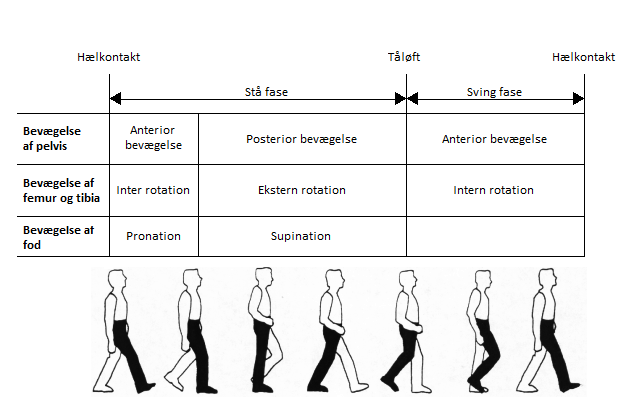
\includegraphics[width=0.9\textwidth]{figures/knaet}
\caption{Viser bevægelse af pelvis, femur og tibia samt foden ved forskellige faser under gang \citep{orthopedics2016}.}
\label{fig:knaet}
\end{figure} 

\noindent
Knæleddet vælges som udgangspunkt for et muligt body augmentation-system i form af et exoskelet, da knæleddet er et hængselled og derfor har et begrænset antal frihedsgrader. Knæleddet har én frihedsgrad, modsat andre mere komplekse led, hvilket gør, at leddet kun kan bevæge sig i én akse \citep{martini2012}. 
Det antages derfor, at knæleddet er et af de led, som er simplest at opbygge et system omkring. 
Hvis der kan laves et exoskelet omkring knæleddet, vil det kunne antages, at samme princip kan muliggøres ved henholdsvis hofte- og ankelleddet, hvorved gangfunktionen kan opretholdes.

\subsection{Knæets opbygning}
Knæet består af tre separate ledforbindelser. To, der er forbundet mellem femur og tibia, samt en mellem patella og femur, hvilket fremgår af \autoref{fig:knae_anatomi}. 

\begin{figure}[H]
\centering
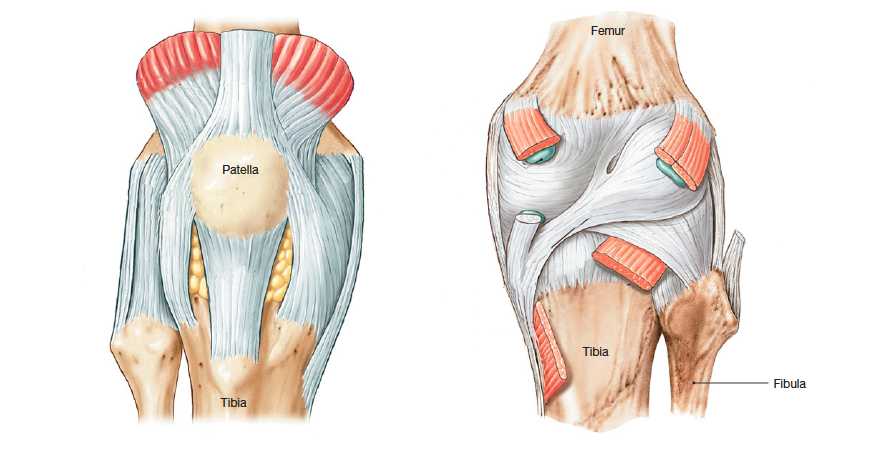
\includegraphics[width=0.8\textwidth]{figures/knae_anatomi}
\caption{Knæets anatomiske opbygning samt knæets forreste og bagerste korsbånd. \citep{aaos2014}.}
\label{fig:knae_anatomi}
\end{figure} 

\noindent
Ud over de tre separate ledforbindelser stabiliseres knæet af syv ledbånd. Ét af de syv ledbånd er patellarsenen, som er ansvarlig under extension af knæet. Derudover strækker to ledbånd sig mellem femur, tibia og fibia, hvilket er med til at styrke knæleddets overflade posteriort. 
Inde i ledkapslen befinder det forreste korsbånd, Anterior Cruciate Ligament (ACL), og det bagerste korsbånd, Posteior cruciate ligament (PCL), sig. Disse har til opgave at fastgøre indre knoglefremspring af tibia til knoglefremspringet på femur. 
Korsbåndene har til opgave at begrænse anteriore og posteriore bevægelser af femur og er med til at opretholde retningen af knoglefremspringene. 
Det tibiale kollaterale ligament forstærker den mediale flade af knæleddet, og det fibulære kollaterale ligament forstærker sidefladen. Disse ligamenter anvendes kun ved fuld ekstension af knæleddet \citep{martini2012}.

\subsection{Knæets funktion}
Ved gang aktiveres quadricepsmusklerne, der sidder anteriort på femur, og hasemusklerne, der sidder poseriort på femur. Nogle af disse muskler fremgår af \autoref{fig:laarmuskler}. Quadricepsmusklerne består af rectus femoris, vastus intermedius, vastus medialis og vastus lateralis. 
Hasemusklerne består af biceps femoris, semitendinosus og semimembranosus. 
Ved bevægelse foretager quadriceps- eller hasemusklerne ekstension eller fleksion, hvorved de fungerer som hinandens agonister eller antagonister under bevægelse \citep{martini2012}. 

\begin{figure} [H]
\centering
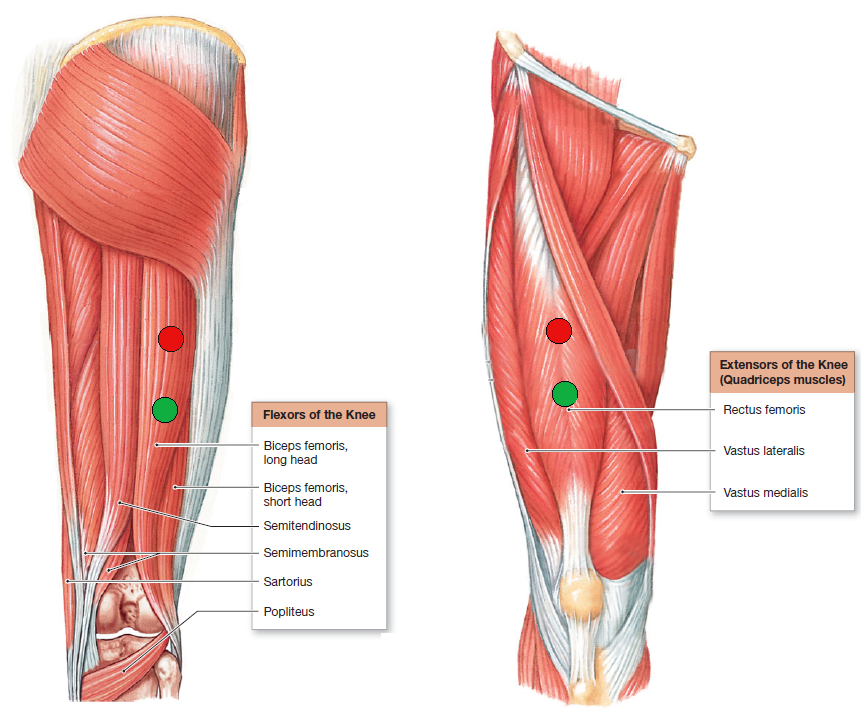
\includegraphics[width=0.9\textwidth]{figures/laarmuskler}
\caption{Viser rectus femoris, vastus lateris, biceps femoris, semimembranosus og patella  \citep{martini2012}.}
\label{fig:knaet}
\end{figure} 


Som tidligere nævnt anvendes hofte, knæ og ankler under gang. Udover disse led er kropsposituren og sving af leddene afgørende for gangfunktionen. Det fremgår af \autoref{fig:knaet}, hvordan de forskellige led udfører fleksion, ekstension og ændres fra ekstension til neutral bevægelse under gang \citep{martini2012}.

\subsubsection{Knæets funktion under en squat-øvelse} \label{sec:knaeled_squat}
% mere om, at det kun er lårets muskulatur, der benyttes under squat
Den dynamiske squat-øvelse er en udbredt træningsøvelse, som kræver styrke i flere muskelregioner. Squat aktiverer primært hofte-, lår- og rygmuskulaturen, som alle er primære muskler under gang, løb, spring og løft. Herudover anvendes squat som et redskab til rehabilitering af knæet, hvilket skyldes den måde, som knæet belastes under squat \citep{escamilla2001}. 

Knæets funktion for bøjningen af benet kan dermed ses ved udførelse af en squat-øvelse. En squat-øvelse udføres ved at stå i en oprejst position med knæ og hofte fuldt udstrakt. Herefter udføres en squat-øvelse i en kontinuerlig bevægelse, indtil den ønskede dybde nåes, hvorefter der udføres en kontinuerlig bevægelse tilbage til oprejst position \citep{escamilla2001}. En illustation af en squat-øvelse ses på \autoref{fig:squat}.

\begin{figure}[H]
\centering
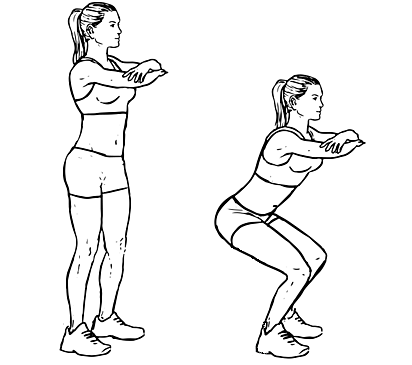
\includegraphics[width=0.5\textwidth]{figures/squat.png}
\caption{En illustration af udførelse af en halv squat-øvelse. Til venstre ses udgangspositionen, og til højre ses en halv squat-øvelse \citep{squat2015}.}
\label{fig:squat}
\end{figure}

\noindent 
Squat-øvelser kan udføres med varierende fleksion af knæet. De mest anvendte varianter af øvelsen er halv eller fuld squat. En halv squat-øvelse udføres indtil lårene er parallelle med jorden, hvilket svarer til en fleksion af knæet fra omkring $90-180^{\circ}$. En fuld squat-øvelse udføres indtil det posteriore del af låret og læggen kommer i kontakt med hinanden. Den fulde squat-øvelse anbefales mere trænede personer, hvorfor den halve squat-øvelse typisk er foretrukket til genoptræning af knæet \citep{escamilla2001}.

Ved udførelse af en squat-øvelse aktiveres blandt andet musklen rectus femoris. Aktiviteten i rectus femoris, og de resterende quadricepsmuskler, er størst ved $90-100^{\circ}$ vinkel af knæleddet \citep{schoenfeld2010}. 
Fra udgangspositionen for squat-øvelsen, der illustreres på \autoref{fig:squat}, befinder personen i en oprejst posistion med en vinkel på $180^{\circ}$ over knæet. Ved udførelse af en squat-øvelse vil muskelaktiviteten i rectus femoris være progressivt stigende indtil en vinkel over knæet på $90-100^{\circ}$ opnås. Idet der returneres til udgangspositionen, vil muskelaktiviteten være progressivt faldende \citep{escamilla2001}. 

%Biceps femoris aktiveres ved en $45^{\circ}$ fleksion af knæleddet, mens rectus femoris aktiveres ved en $80-90^{\circ}$ fleksion, hvorefter aktiviteten i musklerne er konsistent \citep{schoenfeld2010}. 


%Under en squat-øvelse aktiveres vastus intermedius, vastus medialis samt vastus lateris mere, da disse muskler er én ledmuskel, end rectus femoris der er en to-ledsmuskel \fxnote{hvorfor aktiveres én-ledsmuskler mere end to-ledsmuskler - jeg kan ikke finde det med hasemusklerne i den kilde der står til afsnittet?}.
%der er forbundet mellem femur, tibia og patella. Knæet har fire ledbånd. To af disse er side-ligamenterne, der sidder omkring knæleddet. De resterende to er korsbåndene, der sidder på skrå inden i knæet.
%Knæet fire ledbånd sikrer stabilisering af knæet og sørger for at knoglerne bevæger sig rigtigt.  Det er knæleddet, der gør det muligt for kroppen at kunne udføre aktiviteter som at kunne gå, løbe, og eksempelvis squatte. Ved gang aktiveres både quadriceps musklerne (rectus femoris, vastus intermedius, vastus medialis, vastus lateralis) der sidder anteriort for låret samt hamstring musklerne (biceps femoris, semitendinosus, Semimembranosus), der sidder posteriort for låret og kontraherer med quadriceps musklerne. 


% !TeX spellcheck = da_DK
\subsection{Problemafgrænsning}
I dette projekt fokuseres der på ALS patienter samt muligheden for opretholdelse af kropsfunktioner ved benyttelse af body augmentations hjælpemidler. 

Da ALS patienter oplever progressiv svind af deres muskler, har dette indflydelse på deres selvstændighed, da de bl.a. gradvist mister kontrollen over deres legemesdele. Da der kun eksisterer palliative behandlinger til ALS patienter fokuseres der på at afhjælpe deres fysiske mangel ved brug af et exoskelet som aflastning. Dette system kræver minimal fysisk indstat at anvende, hvilket er passende til den typiske ALS patient. 
Ved opretholdes af de fysiske funktioner vil dette ligeledes have en positiv effekt på den sundhedsrelateret livskvalitet, da dette vil kunne resultere i en større selvstændighed. Der er dog igen garanti på at det vil gavne den overordnede livskvalitet hos ALS patienten.  

Idet ALS vil resultere i, at patienten mister evnen til at kunne gå, fokuseres der på at opretholde denne funktion. Til dette er det fremhævet, at knæet er det vigtigste led i forhold til at kunne gå. Dertil vælges der at tages udgangspunkt i knæleddet, hvor musklerne omkringliggende knæet afhjælpes ved anvendelse af et exoskelet.

\subsection{Problemformulering}
Hvordan kan et exoskelet anvendes over et knæled, med henblik på, at ALS patienter skal opretholde deres evne til at gå 
%%-----------------------System udvikling-------------------------
\chapter{Systemudvikling} 
\section{Systembeskrivelse}
Der ønskes, som tidligere nævnt, at udvikle et system, der har til formål at aflaste musklerne omkring knæleddet under udførelse af en statisk squat-bevægelse ved brug af et exoskelet. Dette gøres for at aflaste patienterne med henblik på at kunne undgå kørestol i tidlige stadier af ALS. Systemet skal kunne opsamle signaler fra lårmusklerne; quadriceps og hamstring. Disse signaler skal behandles og omsættes til aktivitet i en prototype af et exoskelet, som skal udføre en tilsvarende bevægelse, men også have mulighed for forstærkning af signalet, så mindre muskelkraft også vil kunne udløse denne bevægelse. Ud over aktiviteten i musklerne skal exoskelettet kunne begrænse bevægelse i visse retninger, så det herved er muligt at rette leddets position, hvis dette bevæger sig uønsket\fxnote{har vi snakket om dette?}. Af denne grund skal systemet være i stand til at måle muskelaktivitet i quadriceps og hamstring samt den aktuelle vinkel i knæleddet. Derudover skal systemet være brugervenligt ved at være kompakt, mobilt og ikke generende over for brugeren.

\subsection{Krav til systemet} 
\begin{itemize}
\item Systemet skal registrere muskelaktivitet og ledvinkler
\item Systemet skal kunne overføre data trådløst til en computer
\item Systemet skal kunne udmundes(bedre ord?) i en prototype af et exoskelet
\item Systemet skal være batteridrevet
\item Systemet skal være sikkert og ikke til gene for brugeren
\item Systemet skal kunne indikere, hvis der ikke er strøm nok til at virke optimalt \fxnote{er dette et vigtigt punkt?}
\item Systemet skal kunne give feedback og derved sørge for, at brugeren befinder sig inden for følgende specifikationer:\fxnote{igen: har vi snakket om dette?}
\begin{itemize}
\item XX antal grader?
\item XX antal grader?
\end{itemize}
\end{itemize}

\fxnote{Punkterne står virkelig tæt på teksten - kan vi ændre på det?}

\subsection{Blokdiagram}\fxnote{ændr feedback til prototype, tilføj måske patienten}
\begin{figure}[H]
\centering
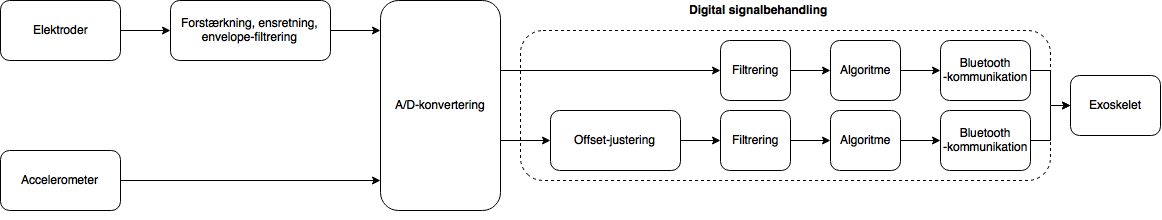
\includegraphics[width=0.4\textwidth]{figures/blokdiagram.png}
\caption{Systemets opbygning.}
\label{fig:blokdiagram}
\end{figure}

%I dette projekt er der valgt at udarbejde en prototype, som har til formål at sørge for at knæledddet forbliver inden for en bestemt position. 
I dette projekt er der valgt at udarbejde en prototype, som har til formål at bøje knæleddet, når lårets muskler kontraherer. Opbygningen af systemet fremgår af \autoref{fig:blokdiagram}. Der anvendes to sensorer, EMG og accelerometer, til at opsamle biologiske signaler, For at registrere muskelaktivitet anvendes en EMG-sensor og en EMG-forstærker, der har til formål at forstærke den muskelaktivitet, der opsamles. Accelerometeret anvendes for at give systemet et input om, knæleddet vinkles  under udøvelsen af en statisk squat. Det opsamlede signal sendes herefter videre til den digitale del af systemet, hvilket er bestående af et Bluetooth Low Energy Pioneer kit (CY8CKIT-042-BLE), som opfanger de biologiske signaler og overfører dem trådløst til en CySmartUSB BLE Dongle sat i en computer, som kan kommunikere med prototypen af exoskelettet i LEGO Mindstorms. 



%%\subsection{Elektromyografi}
%EMG er en målemetode, som måler elektrisk aktivitet genereret af musklerne \citep{chowdhury2013}. 
%En EMG-måling dækker over et samlet antal potentialer fra måleområdet, idet der aktiveres mange muskelfibre \citep{keenan2012}. \fxnote{Ved ikke, om der skal skrives noget om, at muskelfiberne inaverers af motorneuroner, og at mængden af muskelfibre pr. motorneuron afhænger af musklen og dens funktion = det ville være godt, inddrag lidt ALS - KOMMENTAR: lige nu syntes vi ikke at der er relevant}

%Der kan anvendes to forskellige typer af EMG-målinger. Den ene er en ikke-invasiv metode, der kaldes overflade-EMG, og den anden er en invasiv metode, intramuskulær EMG \citep{chowdhury2013, keenan2012}. Hertil anvendes sidstnævnte i dette projekt. 
%Ved generel anvendelse af EMG-målinger, benyttes frekvensområdet ved $10-500~Hz$, hvorfor signaler uden for dette frekvensområde kan betegnes som støj \citep{morre2003, keenan2012}.  

%Denne metode kan påvirkes af flere artefakter, som bevægelsespåvirkning og støjpåvirkning fra elnettet ($50~Hz$) \citep{keenan2012}.
%Ligeledes kan der ved EMG-målinger fremkomme elektrisk støjpåvirkning fra omkringliggende muskler i forhold til området, der måles på. Dette betegnes som crosstalk \citep{keenan2012}. 

\subsection{Elektromyografi}
Til behandling af EMG-signalet, anvendes Muscle Sensor V3, der fremover refereres som 'EMG-forstærker'. Denne komponent måler en differens af de elektriske potentialer der måles gennem elektroderne. EMG-forstærkeren overholder de opstillede krav, og kan anvendes direkte med mikrokontrolleren. EMG-forstærkeren består af en intrumenteringsforstærker, et passivt højpasfilter, en full-wave rectifier, et aktivt lavpass filter og en justerbar forstærker \citep{advancertech2013}. 

En illustration af, hvordan EMG-forstærkeren behandler et inputsignal fremgår af \autoref{fig:sinussignal}.
\begin{figure}[H]
\centering
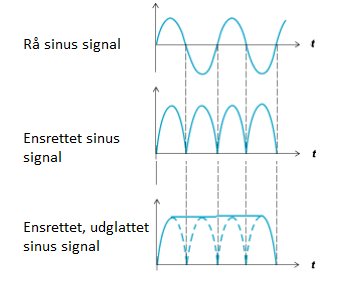
\includegraphics[width=0.6\textwidth]{figures/sinussignal.png}
\caption{Tre sinussignaler. Henholdsvis et råt, ensrettet og ensrettet samt udglattet. \citep{advancertech2013}.}
\label{fig:sinussignal}
\end{figure}

Med udgangspunkt i \autoref{fig:sinussignal} ses signalet som sinuskurven. Hertil passerer det højpasfilteret der dæmper DC støjen og dermed offsettet i signalet. Dette ses som signalet sinuskurven der svinger omkring 0, og er nødvendig for at ensretningen viker efter hensigten. Dernæst ensrettes signalet, således de negative værdier inverteres, og at der kun er svingninger i positiv retning. Herefter fortages et envalope, hvilket ses som det udglattede signal, hvortil der er beregnet en knækfrekvens på $1,94~Hz$, ud fra \autoref{eq:lavcutfre}. 

\begin{equation}\label{eq:lavcutfre}
f_c = \frac{1}{2 \pi C R} = \frac{1}{2 \pi \dot 1 \dot 10^{-6}F \dot 80,6 \dot 10^3\Omega} = 1,94~Hz
\end{equation}

EMG-forstærkeren har en minimum spændingsforsyning på $\pm 3~V$ samt en maksimal spændingsforsyning på $\pm 30~V$. Herudover er der mulighed for at justere gain med en faktor fra 0,002 til 20,700. \citep{advancertech2013}. 





%Synes ikke det passer ind her? Er det ikke meningen dette skal være mere overordnet, og så specificerer vi os senere til hvordan vi vil måle, sådan til vores forsøg?
%Den ene elektrode placeres over enten rectus femoris eller vastus intermedius (sidder under rectus femoris) og den anden elektrode placeres over biceps femoris. Reference elektroden placeres ved??.. 


%Støj kan reduceres ved at placere en 0.1 mikro f capacitor i nærheden, det er dog nødvendigt at tilføje mere, hvis der er 50 KHz støj, da det vil kunne resultere i fejl i accelerations målingen. Støjens tæthed vil forminskes i takt med at forsyningsspændingen forøges.
%Fase sensitiv demodulation teknikker er anvendt for at bestemme magnituden samt accelerationens retning. Demodulator outputtet er forstærket og bragt igennem en 32 k ohm modstand. – noget med det forebygger aliasing 
%  - Jeg ser dette som 'ligegyldigt' nu, da det handler om kondensator og støj. Kan ikke se hvorfor det skal bruges (endnu) måske skal det bruges efter vi har lavet pilotforsøg, hvis der viser sig meget støj






%\subsection{Accelerometer}
Et accelerometer er en elektromekanisk enhed, som både kan måle statisk og dynamisk accerleration. Den statiske acceleration kan være tyngdekraften, hvortil det er muligt at bestemme orienteringen af accelerometeret i forhold til jorden. De dynamiske kræfter såsom bevægelse, stød og vibrationer, gør det muligt at analysere accelerometeres bevægelse samt hastighed. 

I dette projekt anvendes accelerometeret ADXL335Z, som har pin konfigurationen, som kan ses på \autoref{fig:acc_pin}. Accelerometeret er en 3-aksialt sensor, som har et arbejdsområde på minimum $\pm$ $3~g$, og et output som spænding. Det analoge output signal er proportionelle med accelerationen \citep{analogdevices2010}. 


\begin{figure}[H]
\centering
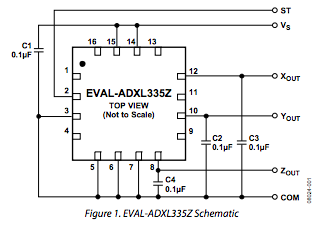
\includegraphics[width=0.6\textwidth]{figures/acc_pin.png}
\caption{Pin konfiguration af accelerometer ADXL335}
\label{fig:acc_pin}
\end{figure}

\noindent
Accelerometeret har en single-supply spændingsforsyning, som ligger mellem $1,8 - 3,6~V$, denne er reguleret til $XX~V$ via tilkobling af en regulator \fxnote{afhænger af hvad Jan sætter regulatoren til}. Offsettet er afhængig efter spændingsforsyningen, men ligger ved $XX~V$ på $XX~V$, denne beregnes som det halve af spændingsforsyningen. Båndbredden og støjen varierer for akserne. For x og y-aksen ligger båndbredden mellem $0,5 - 1.600~Hz$ og støjen normalt på $150~\mu g/\sqrt{Hz}$ RMS, mens båndbredden for z-aksen ligger mellem $0,5 - 550~Hz$ og støjen normalt på $300~\mu g/\sqrt{Hz}$ RMS. \fxnote{Den spektrale effekttæthed måles i $\mu g/$ og dividere dette med kvadratroden for båndbredden for signalet $\sqrt{Hz}$, hvilket giver RMS af accelerationsstøjen ved en temperatur på $25^\circ$C}. 

Da accelerometeret er ratiometrisk, hvilket vil sige at outputtet er direkte propotienelt med input, afhænger sensitiviteten ligesom offsettet af spændingsforsyningen. Ved $XX~V$ spændingsforsyning, ligger forsyningen på $XX~mV/g$ med en tolerance på $XX~\%$, hvor outputimpedansen er $XX~K\omega$ med en afvigelse på $XX~\%$. 

\begin{figure}[H]
\centering
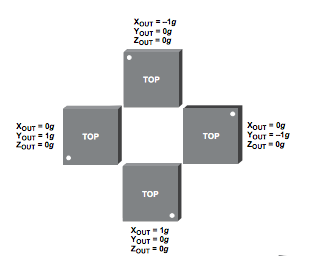
\includegraphics[width=0.8\textwidth]{figures/acc.png}
\caption{Accelerometeret, ADXL335Z, påvirkning i de forskellige akser}
\label{fig:acc}
\end{figure}

\noindent
Ved hældning af accelerometeret vil der ske en acceleration i forhold til tyngdekraften, afhængig af planet samt retningen som det hældes i. Dette fremgår af \autoref{fig:acc}. Herved vil der ske en ændring i spændingen fra referencepunkt ved en hældning på $0^{\circ}$\fxnote{Jeg forstår ikke den her sætning}. Hvis accelerometeret eksempelvis befinder sig i den øverste situation på \autoref{fig:acc}, påvirkes x-aksen med $-1~g$. Denne sammenhæng og derved patientens hældning kan udtrykkes ved følgende ligning:

\begin{equation}
	V_{out} = V_{offset} + sensitiviteten \cdot \sin(vinklen) \\
\end{equation}


%Støj kan reduceres ved at placere en 0.1 mikro f capacitor i nærheden, det er dog nødvendigt at tilføje mere, hvis der er 50 KHz støj, da det vil kunne resultere i fejl i accelerations målingen. Støjens tæthed vil forminskes i takt med at forsyningsspændingen forøges.
%Fase sensitiv demodulation teknikker er anvendt for at bestemme magnituden samt accelerationens retning. Demodulator outputtet er forstærket og bragt igennem en 32 k ohm modstand. – noget med det forebygger aliasing 
%  - Jeg ser dette som 'ligegyldigt' nu, da det handler om kondensator og støj. Kan ikke se hvorfor det skal bruges (endnu) måske skal det bruges efter vi har lavet pilotforsøg, hvis der viser sig meget støj
\section{Løsningsstrategi}
%Intro til hvad der skal være hjernen i systemet.
Til dette system benyttes komponenter fra Cypress's CY8CKIT-042-BLE udviklingssæt. 
Ud fra dette sæt er der udvalgt de nødvendige komponenter, så der kan fortages analog til digital konvertering af de signaler, der måles via sensorerne i \autoref{sec:sensorer}. Yderligere skal systemet være i stand til at kommunikere trådløst med andre enheder.   

\begin{figure}[H]
\centering
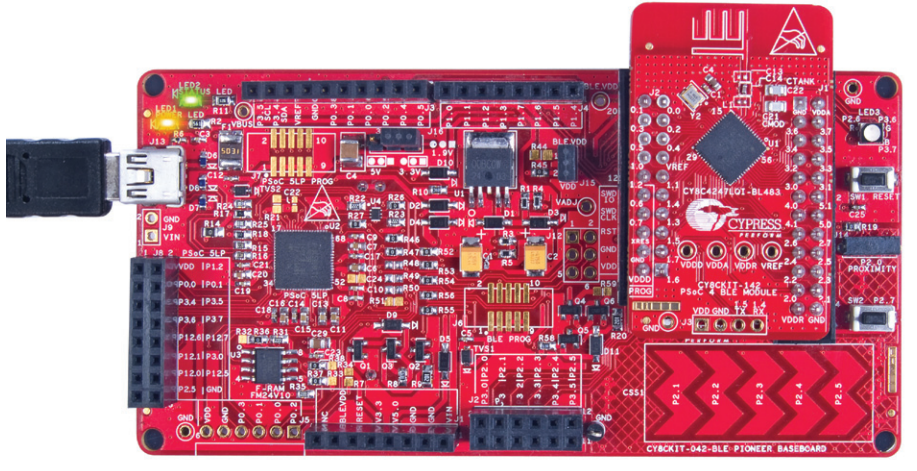
\includegraphics[width=0.5\textwidth]{figures/CY8CKIT-042.png}
\caption{CY8CKIT-042 BLE Pioneer baseboard, samt CY8CKIT-142 PSoC 4 BLE modulet \citep{cypresspsoc2015}.}
\label{fig:CY8CKIT-042}
\end{figure}

I \autoref{fig:CY8CKIT-042}, ses de valgte komponenter, der består af et CY8CKIT-042 BLE Pioneer baseboard og et CY8CKIT-142 PSoC 4 BLE modul. Baseboardet er platformen, hvorpå sensorerne vil blive tilkoblet, og hvor de analoge signaler konverteres til digitale signaler. Baseboardet har mulighed for tilkobling af en spændingsforsyning, bestående af et $3~V$ knapcelle batteri, eller via mikro USB tilslutningen \citep{cypressguide2014}. Der er mulighed for udvidelse af baseboardet, ved anvendelse af moduler fra Cypress, samt Arduino shields eller 6-pins Digilent Pmod udvidelseskort \citep{cypressguide2014}. 
\\


\subsection{Analog til digital konvertering}


\subsection{Trådløs kommunikation}
For at kunne kommunikere trådløst benyttes CY8CKIT-142 PSoC 4 BLE, der et Cypress BLE modul. Kommunikationstypen er Bluetooth Low Energy (BLE) \citep{cypressguide2014}, der er en power-effektiv (dansk ord for power???) form for Bluetooth-teknologi. Bluetooth er en standard for kortdistance trådløs teknologi, som muliggør kommunikation mellem flere enheder gennem radiobølger. Dette betyder, at systemet benytter mindre batteri på Bluetooth-kommunikationen, end almindelig Bluetooth gør. Af denne grund kan der benyttes små batterier, uden det bliver nødvendigt at skifte dem ofte \citep{gupta2013}. 
CY8CKIT-142 PSoC 4 BLE har en operationsfrekvens på $2,4~GHz$ \citep{cypressguide2014}. 
\\

Ud over de to mikrocontrollere til det endelige system, benyttes en BLE-dongle, der giver mulighed for at en computer kan kommunikere trådløst med systemet. Dette tillader således trådløs test og debugging af systemet. BLE-donglen forsynes via USB-porten på den givne computer med $5~V$ \citep{cypressguide2014}. 
\\

Til at programmere og debugge mikrokontrollerne, benyttes det tilhørende Cypress software, PSoC Creator 3.3. 

\fxnote{C programmering - programmering}

%Systemet vil består af et baseboard, hvortil signalet fra de forskellige sensorer vil blive tilsluttet. De anvendte sensorer i dette system kan læses i afsnit ??. Systemet har yderligere mulighed for at blive udvidet med arduinu shields og 6-pins Digilent Pmod udvidelses kort \citep{cypressguide2014}. Baseboardet kan forsynes via et 3 V kanpcelle batteri, eller via USB forbindelse. 

%OPerationsspændinger 1,9 V, 3 V, 3,3 V, eller 5 V \citep{cypress2014}. 
%En enhed der benyttes i systemet er Baseboard'et er den primære komponent i dette system, da denne er ansvarlig for databehandling. Baseboard'et kan tilsluttes andre moduler fra Cypress, samt komponenter som for eksempel arduino shields og 6-pins Digilent Pmod udvidelses kort \citep{cypress2014}. Yderligere vil diverse sensorer, anvendt i systemet, blive tilsluttet til baseboard'et, hvortil vil ske en analog-digital konvertering af signalet. Strømforsyningen til baseboard'et består af et 9 V knapcelle batteri, eller ved tilslutning af USB forbindelse.  

%I dette projekt vil baseboardet blive suppleret med et CY8CKIT-142 PSoC \fixme{PSoC: Programmable System-on-Chip} 4 BLE modul til formål at tillade trådløs kommunikation. Kommunikationens typen kaldes for Bluetooth SMART også kendt som Bluetooth Low Energy (BLE) \citep{cypressguide2014}.
%2,4 GHz radio.


%BLE dongle kan tilsluttes en computer, og har en PRoC BLE enhed til kommunikation. Forsynes med 5 V via USB. Dette tilader computeren at kommunikere med systemet, og at teste og debugge systemet.

%Programmerings- og debug værktøjet til det valgte hardware er PSoC Creator 3.3
%%-----------------------Teori-------------------------
\chapter{Teori og design}
%%\section{Analog del}
\section{Opsamling} \label{sec:sensorer}
I systemet benyttes sensorer til at opsamle flere typer data, hvorfra systemet skal agere. Systemet skal være i stand til at opsamle EMG-signaler, hvor der ønskes en repræsentation af energimængden i signalet. For at dette opnås skal systemet envelopefiltreres. Yderligere ønskes at kunne justere forstærkningen, for at kune tilpasse amplituden af EMG-signalet, og dermed gøre systemet mere alsidigt, så det kan benyttes til flere personer. Den justerebare forstærkning vil muliggøre, at ALS-patienter kan benytte systemet i takt med det progressive muskelsvind.
Systemet skal også være i stand til at opsamle signal fra accelerometre, så accelerationen fra to accelerometre kan omregnes til knæets vinkel. 
\subsection{Opsamling af EMG-signaler} \label{sec:EMG_krav}
EMG er en målemetode, som måler elektrisk aktivitet genereret af muskler \citep{chowdhury2013}. 
Som tidligere nævnt i \autoref{sec:ALS} er ALS en neurodegenerativ sygdom, hvor musklen svinder ind med tiden, hvilket resulterer i mindsket muskelaktivitet. Dette påvirker EMG-målingerne, da den elektriske aktivititet hos ALS patienter derfor er mindre.

Almindeligvis kan der anvendes to former for EMG-målinger. Den ene er en ikke-invasiv metode, der betegnes overflade-EMG, og den anden er en invasiv metode, intramuskulær-EMG \citep{chowdhury2013, keenan2012}. I dette projekt anvendes overflade-EMG for at opfylde projektets overordnede krav \autoref{sec:overordnet_krav}, om at være til mindst mulig gene for patienten. Ved overflade-EMG foretages en måling over et samlet antal potentialer fra måleområdet via differensmåling, herved er det muligt at se aktiveringen af muskelfibrene \citep{keenan2012}. EMG har et frekvensområde på $10-500~Hz$, hvorfor signaler uden for dette frekvensområde, betegnes som støj \citep{morre2003, keenan2012}.  

Denne metode kan påvirkes af flere artefakter, som bevægelsespåvirkning og støjpåvirkning fra elnettet, hvilket ligger på frekvenser omkring $50~Hz$. \citep{keenan2012}.
Ligeledes kan der ved EMG-målinger fremkomme elektrisk støjpåvirkning fra omkringliggende muskler i forhold til området, der måles på. Dette betegnes som crosstalk \citep{keenan2012}. 
\vspace{3mm}

\textbf{Krav:}
\begin{itemize}
\item Skal opsamle signaler fra rectus femoris
\item Skal være anvendeligt med overflade elektroder
\item Skal opsamle muskelsignaler i frekvensområdet mellem $10-500~Hz$
\item Skal forsynes med minimum en spænding på $\pm5~V$ 
\item Skal have et justerbart gain, der ikke kan forstærke over ADC'ens arbejdsområde
\end{itemize}
\subsection{Opsamling af accelerometer-signaler}
Et accelerometer er en elektromekanisk enhed, som både kan måle statisk og dynamisk accereleration. Den statiske acceleration er på $1~g$, hvilket svarer til tyngdekraften. Alt efter hvilken retning accelerometeret holdes i, ændres aksen, hvor der måles $1~g$-påvirkning i.
Ud fra dette er det muligt at bestemme orienteringen af accelerometeret i forhold til jorden. De dynamiske kræfter såsom bevægelse, stød og vibrationer, gør det muligt at analysere accelerometeres bevægelse samt hastighed. Ved bevægelse udsættes accelerometeret både for dynamisk og statisk acceleration. Studier har vist, at den højest mulige acceleration ved bevægelse af en arm går fra 0,5 til 2,0 g-påvirkning. Herved forventes dette ligeledes for et ben under en squat-øvelse \citep{bernmarka2002}. I dette projekt måles vinkelen af knæet under en squat-øvelse, derfor vil det være mest hensigtsmæssigt at placere accelerometeret, så det måler i enten X- eller Y-asken. På baggrund af dette vælges Y-aksen.

\vspace{3mm}

\textbf{Krav:}
\begin{itemize}
\item Skal måle på minimum Y-aksen
\item Skal forsynes med en spænding på $3,3~V$
\item Skal måle accelerationer i $\pm2~g$
%\item Skal give output i form af spænding
%\item Skal forsynes af mikrokontrolleren
\end{itemize}
\subsection{Spændingsforsyning} \label{sec:krav_spaending}
Spændingsforsyningen skal være i stand til at forsyne EMG-forstærkeren med en konstant spænding, så en svingende eller faldende spænding ikke vil forstyrre signalet. Da systemet yderligere skal benyttes trådløst, kræves det, at spændingsforsyningen er batteridrevet. EMG-forstærkeren, der bliver udvalgt i \autoref{sec:EMG_krav} kræver en forsyningsspænding på mellem $\pm 3~V$ og $\pm 30~V$, typisk $\pm 5~V$ \citep{advancertech2013}.


\vspace{3mm}
\textbf{Krav:}
\begin{itemize} 
\item Skal kunne forsyne aktive komponenter i den analoge del af kredsløbet
\item Skal kunne levere en jævn spænding
\item Skal kunne give et signal, hvis der ikke leveres en konstant spænding
%\item Skal forsyne mikrokontrolleren
%\item Skal være batteridrevet 
\end{itemize}

%\section{digital del}
\section{Digital del}
\begin{figure}[H]
\centering
\includegraphics[width=1\textwidth]{figures/implementering/Blokdiagram_digital.png}
\caption{Blokdiagrammets digitale del}
\label{fig:blokdiagram_digital}
\end{figure}

\noindent
Efter opsamling af det analoge signal skal dette konverteres til et digital signal, hvorved signal kan behandles digitalt. Den digitale del af systemet er illustreret på \autoref{fig:blokdiagram_digital}. 






\input{rapportAfsnit/eProblemloesning/adc_teori}
\section{Digital filtrering}

Der findes to former for digital filtrering; Infinite Impulse Response (IIR) og Finite Impulse Response (FIR). Der ses hertil både fordele og ulemper ved begge filtertyper \citep{blandford2012}.

FIR-filtre kan altid laves, således de har en lineær fase, og de er altid stabile. FIR-filtre designes ved at benytte eksempelvis frekvenssampling eller en bestemt vindue-type, hvilket giver en overførselsfunktion. Denne overførselsfunktion kan herved benyttes som digitalt filter \citep{blandford2012}. 

I modsætning til FIR-filtre, har IIR-filtre ikke en lineær fase, og de kan være ustabile. Ud over dette har IIR-filtre stejlere sidelobes end et IIR-filter med samme antal koefficienter. Dette betyder, at filteret er mindre hukommelseskrævende og kan arbejde hurtigere. IIR-filtres designprocedure er udledt af den procedure, som de analoge filtre er designet efter. Af denne grund laves IIR-filtre, ligesom analoge filtre, som Butterworth, Chebyshev type 1 og 2 og elliptiske filtre \citep{blandford2012}. 
\\

Da der ønskes at frafiltrere lavfrekvent støj fra det forstærkede, ensrettede og lavpasfiltrerede EMG-signal, vil et IIR højpasfilter være fordelagtigt for at opnå en skarpere hældning i transitionsbåndet. Herudover vil implementering af et FIR-filter kræve for meget af PSoC'en. Under pilotforsøget i \autoref{sec:pilotforsoeg} ...


\subsection{Trådløs kommunikation}\label{sec:traadloes_komm_design}
For at kommunikere trådløst benyttes Cypress BLE modul. Kommunikationstypen BLE \citep{cypressguide2014} er en energi-effektiv variation af Bluetooth-teknologi. Bluetooth er en standard for kortdistance trådløs teknologi, som muliggør kommunikation mellem flere enheder via radiobølger. Dette betyder, at systemet anvender mindre batteri på Bluetooth-kommunikationen, end på almindelig Bluetooth. Af denne grund kan der benyttes små batterier, uden det bliver nødvendigt at skifte dem ofte \citep{gupta2013}. 

\noindent
Til det endelige system benyttes der udover mikrokontrolleren også en BLE-dongle. Dette er etableret for at tillade trådløst kommunikation mellem en computer og mikrokontrolleren, hvortil en illustration kan ses af \autoref{fig:BLE_to_BLE_Dongle}. 

\begin{figure}[H]
	\centering
	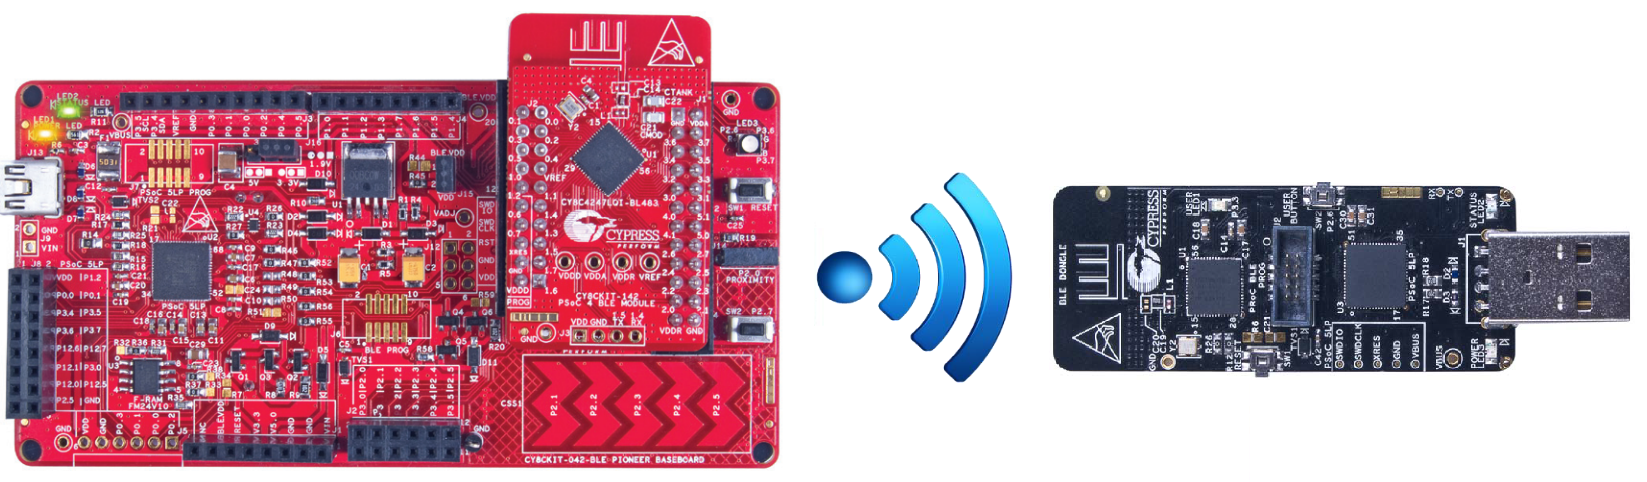
\includegraphics[width=1\textwidth]{figures/BLEToBLEdongle}
	\caption{Illustration af kommunikation mellem mikrokontroller og BLE dongle \citep{cypresspsoc2015, cypressguide2014}.}
	\label{fig:BLE_to_BLE_Dongle}
\end{figure}


Dette tillader således trådløs test, visualisering, og debugging af mikrokontrolleren. BLE-donglen forsynes via USB-porten på den givne computer med $5~V$ \citep{cypressguide2014}. Denne form for BLE-kommunikation anvendes for at kommunikere trådløst med en computer, således en visualisering er mulig. For at systemet senere skal kunne anvendes til ALS-patienter med gang, skal der tages højde for en maksimal forsinkelse, for at systemet kan følge almindelig gang. Gangfunktionen for ALS-patienter varierer alt efter, hvor mange funktioner der er nedsat, eksempelvis vil patienter med luftvejsproblemer gå langsommere. ALS-patienter har en gennemsnitlig gangfunktion på $1,02~m/s$ \citep{hausdorff2000}, hvorfor en forsinkelse på 100 ms vurderes at være acceptabel. Da systemet skal placeres på benet, vurderes det at en kommunikationsrækkevidde på $2~m$ er tilstrækkeligt.
\\

\textbf{Krav:}
\begin{itemize}
\item Mikrokontrolleren skal kommunikere trådløst med en computer
\item BLE-dongle skal forsynes via USB
\item Skal have en maksimal forsinkelse på 100 ms \fxnote{skal denne forsinkelse være større eller mindre?? - HUSK at ændre i brødteksten også!}
\item Skal have en kommunikationsrækkevidde på $2~m$
\end{itemize}
%%-----------------------Implementering-------------------------
\chapter{Implemetering og Test}
\section{Analog del}
\begin{figure}[H]
\centering
\includegraphics[width=1\textwidth]{figures/implementering/Blokdiagram_analog.png}
\caption{Blokdiagrammets analoge del, der implementeres i det følgende afsnit.}
\label{fig:blokdiagram_analog1}
\end{figure}

\noindent
Til implementering af det analoge system, som er illustreret på \autoref{fig:blokdiagram_analog1}, bestemmes der ud fra de opstillede krav i afsnit \autoref{sec:analog_del_krav}, at der skal indgå EMG-signaler og accelerometre til signaloopsamling og behandling. For uden at leve op til de opstillede krav, var disse komponenter til rådighed. Til at forsyne EMG-signaler er der anvendt en spændingsforsyning, som ligeledes er en udleveret komponenten som opfylder kravene stillet i \autoref{sec:krav_spaending}.


%Til implementering af det analoge system, som er illustreret på \autoref{fig:blokdiagram_analog1}, bestemmes der ud fra de opstillede krav i \autoref{sec:analog_del_krav}, at der skal indgå en EMG-forstærker og accelerometre, der introduceres i \autoref{sec:EMG_krav} og \autoref{sec:acc_teori} i implementeringen af systemet. På baggrund af de overordnet krav til systemet er der valgt at anvende EMG og accelerometre, hvorudfra disse krav samt de opstillede krav har medvirket til tilvalg og fravalg af sensorer. Derudover har valget af EMG-forstærker og accelerometre til opsamling af EMG-signal og vinkler været afhængige af, hvilke komponenter der er til rådighed, som opfylder de opstillede krav. 





%\subsection{Elektromyografi}
%EMG er en målemetode, som måler elektrisk aktivitet genereret af musklerne \citep{chowdhury2013}. 
%En EMG-måling dækker over et samlet antal potentialer fra måleområdet, idet der aktiveres mange muskelfibre \citep{keenan2012}. \fxnote{Ved ikke, om der skal skrives noget om, at muskelfiberne inaverers af motorneuroner, og at mængden af muskelfibre pr. motorneuron afhænger af musklen og dens funktion = det ville være godt, inddrag lidt ALS - KOMMENTAR: lige nu syntes vi ikke at der er relevant}

%Der kan anvendes to forskellige typer af EMG-målinger. Den ene er en ikke-invasiv metode, der kaldes overflade-EMG, og den anden er en invasiv metode, intramuskulær EMG \citep{chowdhury2013, keenan2012}. Hertil anvendes sidstnævnte i dette projekt. 
%Ved generel anvendelse af EMG-målinger, benyttes frekvensområdet ved $10-500~Hz$, hvorfor signaler uden for dette frekvensområde kan betegnes som støj \citep{morre2003, keenan2012}.  

%Denne metode kan påvirkes af flere artefakter, som bevægelsespåvirkning og støjpåvirkning fra elnettet ($50~Hz$) \citep{keenan2012}.
%Ligeledes kan der ved EMG-målinger fremkomme elektrisk støjpåvirkning fra omkringliggende muskler i forhold til området, der måles på. Dette betegnes som crosstalk \citep{keenan2012}. 

I dette projekt tages der udgangspunkt i overflade-EMG, hvortil der placeres elektroder på hudoverfladen. 

\subsection{Elektromyografi}
Til behandling af EMG-signalet, anvendes Muscle Sensor V3 fra Advancer Technologies, der fremover vil refereres til som 'EMG-forstærker'. Denne komponent måler en differens mellem de elektriske potentialer, der måles gennem elektroderne. EMG-forstærkeren overholder de opstillede krav, og kan anvendes direkte med mikrokontrolleren. EMG-forstærkeren består af en intrumenteringsforstærker, et passivt højpasfilter, en full-wave rectifier, et aktivt lavpasfilter og en justerbar forstærker \citep{advancertech2013}. 

En illustration af, hvordan EMG-forstærkeren behandler et inputsignal fremgår af \autoref{fig:sinussignal}.
\begin{figure}[H]
\centering
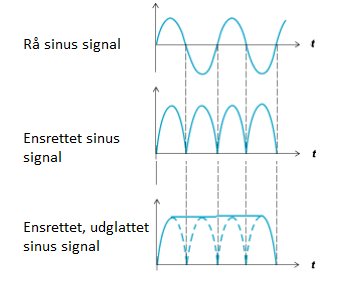
\includegraphics[width=0.6\textwidth]{figures/sinussignal.png}
\caption{Tre sinussignaler. Henholdsvis et råt, ensrettet og ensrettet samt udglattet. \citep{advancertech2013}.}
\label{fig:sinussignal}
\end{figure}

\noindent
Med udgangspunkt i \autoref{fig:sinussignal} opfattes sinuskurven som muskelsignalet. Dette passerer et passivt højpasfilter bestående af en kondensator, der dæmper DC-støjen og dermed offsettet i signalet. Dette betyder, at muskelsignalet centeres omkring 0 på tids-aksen, hvilket er nødvendigt for at få ensretningen til at virke efter hensigten. Dernæst helbølgeensrettes signalet på midterste graf, ved at invertere signalets negative værdier, så signalet udelukkende består af positive værdier samtidigt med at beholde hele dets originale energi. Herefter envelopefiltreres signalet, hvilket ses som det udglattede signal på nederste graf. Til denne filtrering er der beregnet en knækfrekvens på $1,94~Hz$ ud fra \autoref{eq:lavcutfre}. $C$ og $R$ kan i databladet for EMG-forstærkeren aflæses til at være henholdsvis $1 \cdot 10^{-6}~F$ og $80,6 \cdot 10^3~\Omega$ \citep{advancertech2013}. 

% Til udglatningen er der anvendt en bin-integrator, der virker ved at beregne en middelværdi over er given stykke tid. Dette er tilsvarende at der udgregnes en middelværdi af en bestemt mængde data \citep{harb2005}. 

\begin{equation}\label{eq:lavcutfre}
f_c = \frac{1}{2 \pi C R} = \frac{1}{2 \pi \cdot 1 \cdot 10^{-6}~F \cdot 80,6 \cdot 10^3~\Omega} = 1,94~Hz
\end{equation}

EMG-forstærkeren har en minimum spændingsforsyning på $\pm 3~V$ samt en maksimal spændingsforsyning på $\pm 30~V$. Herudover er der mulighed for at justere modstanden heri fra $0,1~\Omega$ til $100~k\Omega$, hvilket giver et justerbart gain fra 0,002 til 20.700 gange. \citep{advancertech2013}. 
\subsection{Implementering af accelerometre}
%Et accelerometer er en elektromekanisk enhed, som både kan måle statisk og dynamisk accerleration. Den statiske acceleration kan være tyngdekraften, hvor det er muligt at bestemme orienteringen af accelerometeret i forhold til jorden. De dynamiske kræfter såsom bevægelse, stød og vibrationer, gør det muligt at analysere accelerometeres bevægelse samt hastighed. 

I dette projekt anvendes der på baggrund af krav opstillet i \autoref{sec:acc_teori} to accelerometre ADXL335Z fra Analog Devices. Accelerometerne er en 3-aksialt sensor, som har et arbejdsområde på minimum $\pm~3~g$, og en spænding som output. Det analoge outputsignal er proportionalt med accelerationen \citep{analogdevices2009}. 

\noindent
Accelerometrene har en single-supply spændingsforsyning, som skal ligge mellem $1,8~-~3,6~V$.  Offsettet er afhængig af spændingen i spændingsforsyningen, da spændingen er $3,4~V$, bliver offsettet $1,7~V$, som er det halve af spændingsforsyningen. Båndbredden og støjen varierer for akserne. For x- og y-aksen ligger båndbredden mellem $0,5 - 1.600~Hz$ og støjen normalt på $150~\mu g/\sqrt{Hz}$ RMS. \fxnote{Den spektrale effekttæthed måles i $\mu g/$. Hvis dette divideres med kvadratroden af båndbredden af signalet $\sqrt{Hz}$, fås RMS af accelerationsstøjen ved en temperatur på $25^\circ$C} \citep{analogdevices2010}. %mens båndbredden for z-aksen ligger mellem $0,5 - 550~Hz$ og støjen normalt på $300~\mu g/\sqrt{Hz}$ RMS. 

Da accelerometrenes output er direkte proportienalt med dets input, afhænger sensitiviteten og offsettet af spændingen i spændingsforsyningen. Ved $3~V$ er sensitiviteten typisk $300~mV/g$ \citep{analogdevices2010}. 


\begin{figure}[H]
\centering
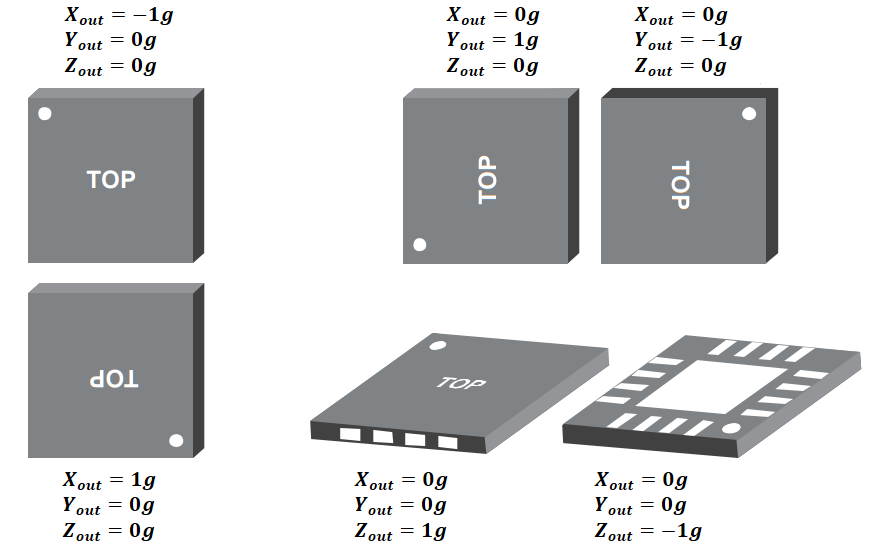
\includegraphics[width=0.85\textwidth]{figures/acc_paavirkning}
\caption{Påvirkning af accelerometeret i forskellige positioner. Til venstre måles accelerometeret lodret, til højre øverst vandret og til højre nederst i plan \citep{analogdevices2010}.}
\label{fig:acc}
\end{figure}

\noindent
Ved hældning af accelerometeret vil der ske en acceleration i forhold til tyngdekraften. Hvilken acceleration, der sker, er afhængigt af plan og hældningens retning. Dette fremgår af \autoref{fig:acc}. Herved vil der ske en ændring i outputspændingen ved en hældning på $0^{\circ}$. Hvis accelerometeret eksempelvis befinder sig i den øverste situation på \autoref{fig:acc}, påvirkes y-aksen med $-1~g$ \citep{clifford2005}. Denne sammenhæng og derved patientens hældning kan udtrykkes ved ligning \autoref{equ:vinkler}, hvor $\phi$ er vinklen i forhold til udgangspunktet for den pågældende akse \citep{clifford2005}.

\begin{equation} \label{equ:vinkler}
	V_{out} = V_{offset} + sensitivitet \cdot \sin(\phi) \\
\end{equation}

\noindent

\subsection{Digital del}

\begin{figure}[H]
\centering
\includegraphics[width=1\textwidth]{figures/implementering/Blokdiagram_digital.png}
\caption{Blokdiagrammets digitale del}
\label{fig:blokdiagram_digital1}
\end{figure}

Til implementering af det digitale system, som er illustreret på \autoref{fig:blokdiagram_digital1}, stilles der fra \autoref{sec:digital_del_krav} krav i forhold til implementeringen af ADC, filtrering og trådløs kommunikation. Da mikrokontrolleren er udleveret på dette semester er det et krav at anvende ADC'en på denne samt BLE-modulet, hvorfor A/D-konvertering og den trådløse kommunikation implementeres på denne. Derudover testes det, hvorvidt de forskellige filtre filtrere det uønskede signal fra. 




\subsection{Analog til digital konvertering} \fxnote{Dette afsnit er meget uklart - omformuler og uddyb}
Mikrokontrolleren indeholder en SAR ADC, som gør det muligt at konvertere det analoge signal til et digital. Det er muligt at konfigurere op til 8 analoge kanaler og læse dem samlet eller kun en enkelt indgang ad gangen. Der kan vælges mellem at anvende 8, 10 og 12 bit og kan sample op til 1 Million Samples Per Sekund (MSPS) med en opløsning på 12 bit. SAR ADC'en understøtter single ended og differentiale indgange. Derudover er det muligt at tilføje en indsprøjtning kanal ved scanningssekvens med firmwarekontrol ved runtime. ADC'en kan den sættes op så den i hardware udfører en gennemsnitsberegning. \citep{ADC2014}


%\input{rapportAfsnit/eProblemloesning/Implementering/} trådløs kommunikation indsættes her
%\input{rapportAfsnit/eProblemloesning/Implementering/} indledning til filtering her??
\subsubsection{IIR-lavpasfilter}
Det ønskede 2. ordens IIR-lavpasfilter er udarbejdet ud fra kravene opstillet i \autoref{sec:lavpas_krav}  og implementeres digitalt ved anvendelse af MATLAB og PSoC. 
Teorien hertil er beskrevet i \autoref{sec:teori_filter}. 
Ved implementering af dette filter benyttes MATLAB for således at beregne a- og b-koefficienterne for et Butterworth filter. 
For beregning af filtret anvendes \autoref{eq:iirfilt}. 

Koefficienterne fremgår af \autoref{tab:koeff_lav}. Dertil defineres a- og b-koefficienterne samt filterlængden i PSoC, hvorefter disse anvendes til programmering af lavpasfiltret. 

\begin{table}[H]
\centering
\begin{tabular}{|c|c|c|c|}
\hline
\textbf{a} & 1,0000 & -1,8890 & 0,0015 \\ \hline
\textbf{b} & 0,0015 & 0,0029  & 0,0015 \\ \hline
\end{tabular}
\caption{De udregnede a- og b-koefficienter for et Butterworth filter.}
\label{tab:koeff_lav}
\end{table}
\subsection{Implementering af et moving average filter}
Det ønskes at implementere et moving average filter ved anvendelse af MATLAB samt PSoC. Koefficienten, a, defineres til at have en værdi på 1, da denne er konstant ved FIR-filtre. Koefficienten, b, defineres ved at dividere a med filterlængden. Disse koefficienter findes i MATLAB og bliver overført til moving average filteret programmeret i PSoC. 

\subsection{Vinkelberegning}\label{sec:imp_vinkler}
I \autoref{sec:test_acc} fremgår det, at der er lineær sammenhæng mellem vinklerne over tid. Det er derfor muligt at udføre en lineær interpolation over dataen af målinger fra accelerometrene i forskellige vinkler. På denne måde er det muligt at bestemme, hvilken som helst vinkel for en tilsvarende spænding. Da målingerne af linearitet, målt i \autoref{sec:test_acc}, er foretaget med Ni USB-6009 stemmer spændingerne ikke overens, når det samples på mikrokontrolleren. Derfor udføres der en ny måling af linearitet med mikrokontrolleren, hvor spændingen i de forskellige vinkler er målt. Efterfølgende er der aflæst et offset, som er trukket fra, for at centrere signalet omkring 0. Offsettet for accelerometeret placeret på låret er aflæst til $-1003~V$ og accelerometeret placeret på skinnebenet til $-972~V$. De målte spændinger, hvor signalet er offsetjusteret fremgår af \autoref{tab:vinkelinterval_psoc}. .

%\begin{comment}
%\begin{table}[H]
%	\centering
%	\begin{tabular}{|l|l|l|}
%				%& \textit{Accelerometer placeret på låret} &				
%	\textbf{Interval} & \textbf{Målt spænding} & \textbf{Målt spænding} 	\\ \hline	
%    \textbf{0-10} 			& $0~V$							& $-186~V$   \\ \hline
%    \textbf{10-30} 			& $-31~V$						& $-185~V$	\\ \hline
%    \textbf{30-50} 			& $-67~V$						& $-168~V$	\\ \hline
%    \textbf{50-70} 			& $-126~V$						& $-126~V$	\\ \hline
%    \textbf{70-80} 			& $-168~V$						& $-67~V$	\\ \hline
%    \textbf{80-90} 			& $-185~V$						& $-31~V$	\\ \hline
%    				%& \textit{Accelerometer placeret på skinnebenet} &		
%    	\textbf{Interval} & \textbf{Målt spænding} & \textbf{Målt spænding} 		\\ \hline	
%    \textbf{0-10}			& $0~V$ 							& $-179~V$	    \\ \hline
%    \textbf{10-30}			& $-16~V$						& $-176~V$	 	\\ \hline
%    \textbf{30-50}			& $-52~V$						& $-153~V$		\\ \hline
%    \textbf{50-70}			& $-111~V$						& $-111~V$		\\ \hline
%    \textbf{70-80}			& $-153~V$						& $-52~V$	 	\\ \hline
%     \textbf{80-90}			& $-176~V$						& $-16~V$	 	\\ \hline
%	\end{tabular}
%	\caption{Spændingen målt i vinklerne fra 0 til 90$^{\circ}$ for accelerometrene placeret på både låret og skinnebenet. Den første spænding svarer til start intervallet og den sidste til slutningen afintervallet.}
%	\label{tab:vinkelinterval_psoc}
%\end{table}
%\end{comment}


\begin{table}[]
\centering
\begin{tabular}{|l|c|c|}
         & \textit{Accelerometer placeret på låret}                           & \multicolumn{1}{l}{}                      \\ \hline
Interval & Målt spænding {[}V{]}                                              & \multicolumn{1}{l}{Målt spænding {[}V{]}} \\ \hline
0 - 10   & 0                                                                  & - 31                                      \\ \hline
10 - 30  & - 31                                                               & - 67                                      \\ \hline
30 - 50  & - 67                                                               & - 126                                     \\ \hline
50 - 70  & - 126                                                              & - 168                                     \\ \hline
70 - 80  & - 168                                                              & - 185                                     \\
\hline
80 - 90  & -185                                                               & - 186                                     \\
\hline
         & \multicolumn{1}{l}{\textit{Accelerometer placeret på skinnebenet}} & \multicolumn{1}{l}{}                      \\ \hline
Interval & Målt spænding {[}V{]}                                              & \multicolumn{1}{l}{Målt spænding {[}V{]}} \\ \hline
0 - 10   & 0                                                                  & - 16                                      \\
\hline
10 - 30  & - 16                                                               & - 52                                      \\
\hline
30 - 50  & - 52                                                               & - 111                                     \\
\hline
50 - 70  & - 111                                                              & - 153                                     \\
\hline
70 - 80  & - 153                                                              & - 176                                     \\
\hline
80 - 90  & - 176                                                              & - 179    \\ \hline 
\end{tabular}
\caption{Spændingen målt i vinklerne fra 0 til 90$^{\circ}$ for accelerometrene placeret på både låret og skinnebenet. Den første spænding svarer til start intervallet og den sidste til slutningen afintervallet.}
\label{tab:vinkelinterval_psoc}        
\end{table}

Spændingen er målt for vinklerne fra 0 til 90$^{\circ}$ for accelerometrene placeret på både låret og skinnebenet. Den første målte spænding er for startværdien i intervallet og den sidste spænding er slutværdien i intervallet.

Ud fra de målte værdier i de forskellige intervaller, er der opstillet en funktion indeholdt ifelse-løkker, hvorved det er muligt at vurdere, hvilket interval en given spænding befinder sig i. I hver enkelt løkke anvendes lineær interpolation, som har til opgave at finde en vinkel, der er svarende til en spænding som ligger mellem intervallet og returnerer denne. 

Når der er udført lineær interpolation over dataen skal de målte data fra låret samt skinnebenet ligges sammen for at få den samlede vinkel af, hvor langt personen har bevæget sig, og derved befinder sig i squat-øvelsen. Resultaterne er optaget på mikrokontrolleren og visualiseres i MATLAB, hvilket fremgår af \autoref{fig:acc_imp}.
 

\begin{figure}[H]
\centering
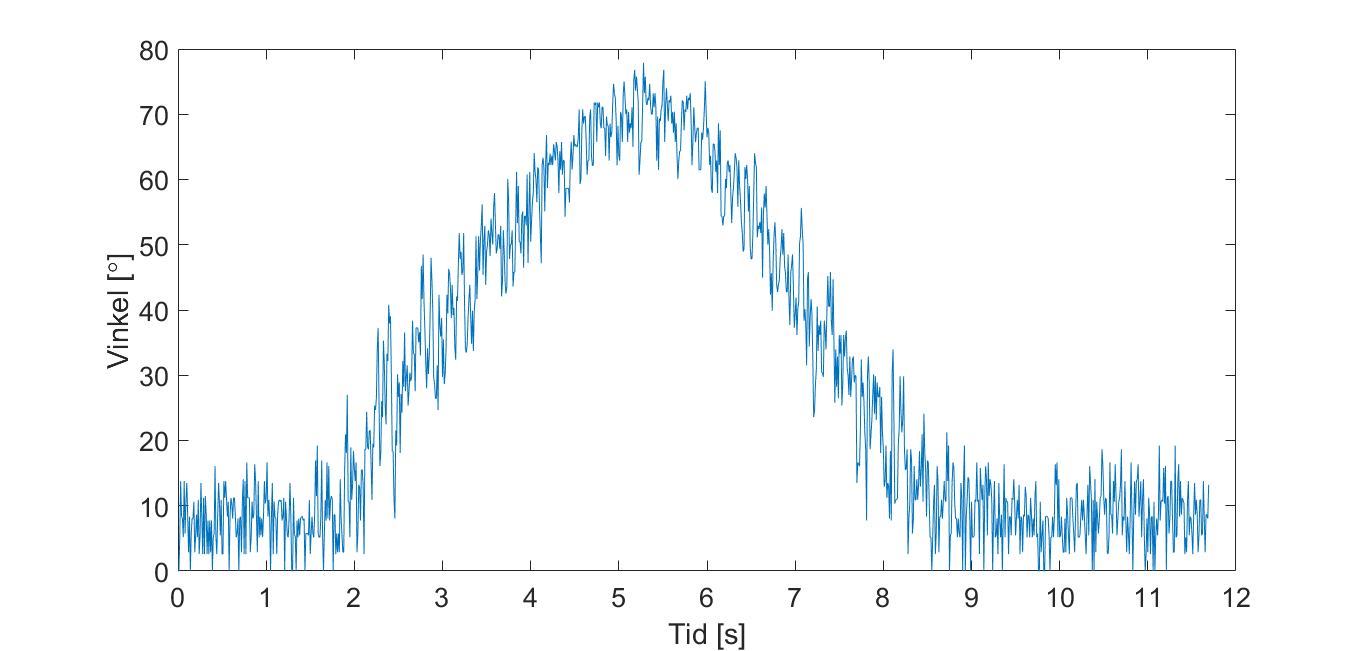
\includegraphics[width=0.8\textwidth]{figures/Pilotforsoeg/accvinkel}
\caption{Samlet vinkler af accelerometrene under udførelse af squat-øvelsen}
\label{fig:acc_imp}
\end{figure}



 %måske skal dette være et andet sted
\section{Flowdigram}
I dette afsnit fremgår implementeringen af systemets blokke \autoref{sec:blokdiagram}. Flowdiagrammer er anvendt for at visualisere opbygningen og sammenhængen mellem blokkene. Flowdiagrammene er opdelt og består af et overordnet, som beskriver hele processen og et initialiserende samt et, der viser EMG-algoritmen. Udover den visualiserende del vil det blive uddybet, hvilke funktioner de enkelte figurer indeholder. Anvendelsen af de forskellige figurer er beskrevet i \autoref{sec:flowhaandtering}.

\subsection{Overordnet flowdiagram}	
Det analoge signal, som optages af de implemterende sensorer skal konverteres fra analogt til digitalt, hvorved det efterfølgende kan implementeres i softwaren. Det overordnede flowdiagram fremgår af \autoref{fig:overordnet_flow}. For at implementering af softwaren vil foreløbe skal der ske et interrupt, som igangsætter de efterfølgende funktioner. Dette igangsætter et timer interrupt, der tæller inden for XX interval. Herefter sker der en intialisering af systemet.

\begin{figure}[H]
\centering
\includegraphics[width=0.6\textwidth]{figures/implementering/overordnet_flow.png}
\caption{Overordnet flowdigram som viser opbyggelsen af det samlede system}
\label{fig:overordnet_flow}
\end{figure}


\subsection{Initialiserende flowdiagram}
I intialiseringsprocessen, der fremgår af \autoref{fig:initialiserende_flow} sker opsætningen af ADC'en, hvorefter det er muligt at se, hvorvidt kravet for det analoge input opfyldes. Ved et analogt input sker en A/D-konvertering, hvor det analoge signal digitaliseres. For at kunne behandle dataen og kommunikere trådløst igangsættes et setup, hvor BLE tilkobes og signalet offsetjusteres. Hvis kravet for det analoge input ikke opfyldes, vil systemet gå i low power mode. Efter setup skal det vurderes, hvorvidt inputtet befinder sig inden for en spænding svarende til 0 til 90 graders vinkel, hvis dette er tilfældet vil signalet starte EMG-algortimen. Hvis inputsignalet ikke er tilstrækkeligt, vil en rød LED lyse og intialiseringsprocessen vil starte på ny. 
\begin{figure}[H]
\centering
\includegraphics[width=0.6\textwidth]{figures/implementering/initialiserende_flow.png}
\caption{Initialiserende flowdigram som viser opbyggelsen af den intialiserende del af systemet}
\label{fig:initialiserende_flow}
\end{figure}

\subsection{EMG-algoritme}
EMG-algoritmen fremgår af \autoref{fig:Emg_algo}. Hvis inputtet svarer til en spændingen mellem 0 til 90 grader vurderes det, hvorvidt muskelaktiviteten er faldende eller stigende. Hvis der ingen muskelaktivitet er, påbegyndes en loop, hvor det igen vurderes om muskelaktiviteten er stigende eller faldende. Hvis der efter 30 sekunder fortsat ingen muskelaktivitet er, afsluttes EMG-algoritmen. Hvis muskelaktiviteten er stigende, vil vinklen blive større, og herved slutter EMG-algoritmen og sender et input videre til BLE, hvorved en fleksion af knæleddet påbegyndes. Hvis muskelaktiviteten er faldende vil viklen blive mindre, hvilket ligeledes slutter EMG-algoritmen og sender et input videre til BLE, hvorved en ektension af knæleddet påbegyndes. 
\begin{figure}[H]
\centering
\includegraphics[width=0.6\textwidth]{figures/implementering/EMG_algo.png}
\caption{EMG-algoritmen viser opbyggelsen af EMG-algortimens del af systemet}
\label{fig:Emg_algo}
\end{figure}



%\iffalse
\begingroup
\raggedright

\bibliographystyle{unsrtnat}
\bibliography{kilder}

\endgroup

%-----------------------Bilag-------------------------
\appendix
\chapter{Bilag}
\section{Pilotforsøg}
%Nirushas udgave
I dette projekt udføres et pilotforsøg for identificering af støj samt andre uønskede signaler ved anvendelse af sensorer. Pilotforsøget danner grundlag for optimering af kravspecifikationerne i de forskellige blokke. Herudover undersøges elektrodernes placering for at opnå det bedst mulige signal under udførelse af en squat-øvelse.
%Signes udgave
I dette projekt udføres et pilotforsøg for identificering af støj samt andre uønskede signaler ved anvendelse af sensorer. Pilotforsøget danner grundlag for optimering af kravspecifikationerne i de enkelte blokke. Derudover undersøges det, hvor elektroderne skal placeres for at opnå det bedst mulige signal under udførelse af en squat-øvelse.


\subsection{Formål}
Der anvendes en EMG-forstærker og et accelerometer som sensorer. På baggrund af dette opstilles følgende formål for de enkelte sensorer.  

\subsubsection{EMG-forstærker}
\begin{enumerate}
\item Opsamling af signal fra rectus femoris og biceps femoris
\begin{itemize}
%Nirushas udgave
\item Identificering af elektrodernes placering
\item Sammenligning af muskelaktivitet under en squat-øvelse 
%Signes udgave
\item Identificere placeringen af elektroder
\item Sammenligne muskelaktivitet oprejst og i en squat-øvelse 

\end{itemize}
\item Identificering af støjsignaler
\end{enumerate}


\subsubsection{Accelerometer}
\begin{enumerate}
%Nirushas udgave
\item Identificering af position under en squat-øvelse
\item Identificering af støjsignaler
%Signes udgave
\item Identificere position af knæleddet siddende i en squat-øvelse
\item Identificere støj ved opsamling af signaler

\end{enumerate}


\subsection{Materialer} 
\begin{itemize}
\item EMG-forstærker
\item Elektroder
\item Desinfektionsservietter
\item Skraber
\item Tusch 

\item Accelerometer ADXL335Z
\item Tape
\item Ledninger

\item Computer
\item CY8CKIT-042-BLE
\end{itemize}

\subsection{Metode}

%Nirushas udgave
For at identificere den bedste mulige elektrodeplacering optages EMG signaler fra forskellige placeringer på de to muskler. 
For at simulere den påvirkning som accelerometeret udsættes for og derved identificere det maksimale og minimale outputsignal roteres accelerometeret i en langsom rotation fra 0 $^{\circ}$ til 90 $^{\circ}$ til både højre og venstre. Herudover måles accelerometerets påvirkning i henholdsvis 0 og 1 g-påvirkning, for at identificere accelerometeres påvirkning og hvorledes dette stemmer overens med databladet. 
For at identificere støj fra EMG forstærkeren optages aktivitet i musklerne under en squat-øvelse.
 
%Signes udgave
For at identificere den bedste placering af elektroder optages EMG-signaler fra forskellige placeringer på de to muskler. 
For at simulere den påvirkning som accelerometeret udsættes for og derved identificere det maksimale og minimale outputsignal roteres accelerometeret i en langsom rotation fra 0 $^{\circ}$ til 90 $^{\circ}$  til både højre og venstre. Herudover måles accelerometeret påvirkning i henholdsvis 0 og 1 g-påvirkning for at identificere accelerometeres påvirkning og hvorledes dette stemmer overens med databladet. 
For at identificere støj fra EMG-forstærkeren optages aktivitet i musklerne i en squat-øvelse.


\subsection{Forsøgsopstilling}
Forsøgsopstilling er for den primære udførelse af forsøget. Nogle af processerne gentages for at kunne sammenligne de forskellige målinger, og derved få et bedre resultat.

%Nirushas udgave
\subsubsection{EMG-forstæker}
Rectus femoris og biceps femoris identificeres, den ønskede placering af elektroderne markeres med tusch. Herefter fjernes eventuelle hår og døde hudceller ved brug af skraber. Huden desinficeres herefter ved brug af desinficeringsservietter og elektroderne påsættes. Den røde ledning påsættes rectus femoris/bicep femoris og den grønne ledning påsættes rectus femoris/bicep femoris. Den sorte ledning påsættes (tibia) og anvendes som referencepunkt.
%Signes udgave
\subsubsection{EMG-forstæker}
Rectus femoris og biceps femoris identificeres, den ønskede placering af elektroderne markeres med tusch. Herefter fjernes eventuelle hår og døde hudceller ved brug af skraber. Huden desinficeres herefter ved brug af desinficeringsservietter og elektroderne påsættes. Den røde ledning påsættes rectus femoris/bicep femoris og den grønne ledning påsættes rectus femoris/bicep femoris. Den sorte ledning påsættes patella og anvendes som referencepunkt.


\subsubsection{Accelerometer}
Accelerometeret påsættes siden af låret, så accelerometer måles i xyz-plan, hvorved der måles i den vertikale retning. Der sørges for,  at accelerometeret befinder sig i 0 g påvirkning ved starten af forsøgets udførelse, hvorved accelerometeret er kaliberet. 

\subsubsection{Opstilling}
\begin{itemize}
\item Identificering af musklerne rectus femoris og biceps femoris 
\item Elektrodernes placering markeres
\item Huden skrabes og desinficeres
\item Elektroderne påsættes
\item Ledningerne påsættes elektroderne
\begin{itemize}
\item Den røde/grønne ledning på rectus femoris
\item Den røde/grønne ledning på biceps femoris
%Nirushas udgave
\item Den sorte ledning/reference på tibia??
%Signes udgave
\item Den sorte ledning/reference på patella \fxnote{positiv/negativ/ground}

\end{itemize} 
\item Accelerometeret på sættes patella ved en 0 g påvirkning i x,y,z retning
\end{itemize}


\subsection{Fremgangsmåde}
Fremgangsmåden udføres XX antal gange, hvorved der på baggrund af målingerne foretages en gennemsnitsværdiberegning.
%Nirushas udgave
\subsubsection{EMG/EMG forstærker}
EMG måling: Squat-øvelsen starter stående, hvorefter forsøgspersonen langsomt udføre bevægelsen og dermed kommer ned i en dybere squat, hvor der undervejs foretages målinger.
%Signes udgave
\subsubsection{EMG/EMG-forstærker}
EMG måling: 10-sekunders målinger trinvist under udførelse af en squat-øvelse. 


\subsubsection{Accelerometer}
Påvirkning i 0 og 90 $^{\circ}$.
Påvirkning af rotation fra 0 til 90 $^{\circ}$ til både højre og venstre.
Optag 30 sekunder ved 0 og 90 $^{\circ}$ .
Optag rotation: baseline 10 sekunder, rotation 10 sekunder, baseline 10 sekunder





\section{Test af accelerometer} 
\label{sec:test_acc}
I dette projekt anvendes to accelerometre, som er beskrevet i \autoref{sec:acc}. Disse anvendes som sensorer til opsamling af acceleration, der giver et outputsignal svarende til en spænding. For at kunne anvende et accelerometer er det vigtigt at kende forskellige tolerancer i forhold til deres datablade, hvorfor et forsøg udføres for at kunne tage højde for disse parametre.

\subsection{Formål}\label{sec:acc_formaal}
Denne test har til formål at identificere en given spændingen for forskellige vinkler. Derudover identificeres %støjsignaler i outputsignalet samt 
offsettet og sensitiviteten for at teste accelerometrenes tolerancer.

\begin{enumerate}
%\item Identificering af støj i outputsignaler for accelerometrene
\item Test af linearitet
\item Identificering af offsettet og sensitiviteten for accelerometrene
\item Identificering af spænding ved forskellige vinkler
\end{enumerate}

\subsection{Materialer}
\begin{itemize}
\item Accelerometre ADXL$335$
\item Tape
\item Vaterpas
\item Breadboard
\item LEGO-model, fremgår af \autoref{fig:vinkeltest}
\item Computer med Scopelogger og MATLAB
\item NI USB-6009
\end{itemize}

\subsection{Metode}
Der opstilles en metode til hvert formål i \autoref{sec:acc_formaal}. Formål 1 opfyldes ved deltest 1, og formål 2 og 3 opfyldes ved deltest 2. 
\begin{enumerate}
%\item Der foretages målinger i accelerometerets tre akser og i de seks positioner som accelerometeret, hvorved støj som accelerometeret påvirkes med kan identificeres
\item Der foretages målinger i accelerometerets tre akser i 11 positioner, hvorved der kan testes for linearitet
\item Der foretages målinger i accelerometerets tre akser i de seks positioner, hvorefter offset og sensitiviteten kan beregnes ud fra målingerne. Offsettet beregnes ud fra accelerometerets 0 g-påvirkning, der måles vinkelret på planet, hvilket svarer til at accelerometeret ikke udsættes for tyngdekraften. Sensitiviteten måles ud fra en 1 g-påvirkning
\item Ud fra målingerne ved 0 og 1 g-påvirkning kan spændingen ved $1^{\circ}$ og $90^{\circ}$ kan beregnes ved \autoref{equ:vinkler}
\end{enumerate}

\subsection{Forsøgsopstilling}
Forsøgsopstillingen udføres på samme måde for begge accelerometre.

\subsubsection{Forsøgsopstilling af deltest 1}
\begin{itemize}
\item Accelerometeret påsættes LEGO-modellen på \autoref{fig:vinkeltest}
\begin{itemize}
\item Accelerometeret indstilles efter fremgangsmåden for hver øvelse som er illustreret i \autoref{sec:vinkel_fremgangsmaade}
\end{itemize}
\item Accelerometeret tilkobles NI USB-6009
\item NI USB-6009 tilkobles en computer
\end{itemize}

\subsubsection{Forsøgsopstilling af deltest 2}
\begin{itemize}
\item Accelerometeret påsættes breadboardet og fastsættes med tape
\item Accelerometeret indstilles, så det er i vater med et vaterpas
\begin{itemize}
\item Accelerometeret placeres efter fremgangsmåden for hver øvelse, hvilket er illustreret i \autoref{sec:acc_fremgangsmaade}
\end{itemize}
\item Accelerometeret tilkobles NI USB-6009
\item NI USB-6009 tilkobles en computer
\end{itemize}

\subsection{Fremgangsmåde}  

\subsubsection{Fremgangsmåde for deltest 1} \label{sec:vinkel_fremgangsmaade}
Hver vinkel måles og samples for hvert accelerometer i hver akse i 10 sekunder ved $100~Hz$, hvilket er det dobbelte af båndbredden for accelerometrene \citep{analogdevices2010}. Målingerne er udført for begge accelerometre i henholdsvis x-, y- og z-aksen, og vinklen ændres ved at justere LEGO-modellen på \autoref{fig:vinkeltest}, så følgende vinkler fremgår af modellen:
\begin{itemize}
\item $0^{\circ}$ til $180^{\circ}$ med $20^{\circ}$'s intervaller
\item $90^{\circ}$  
\end{itemize}


\begin{figure}[H]
\centering
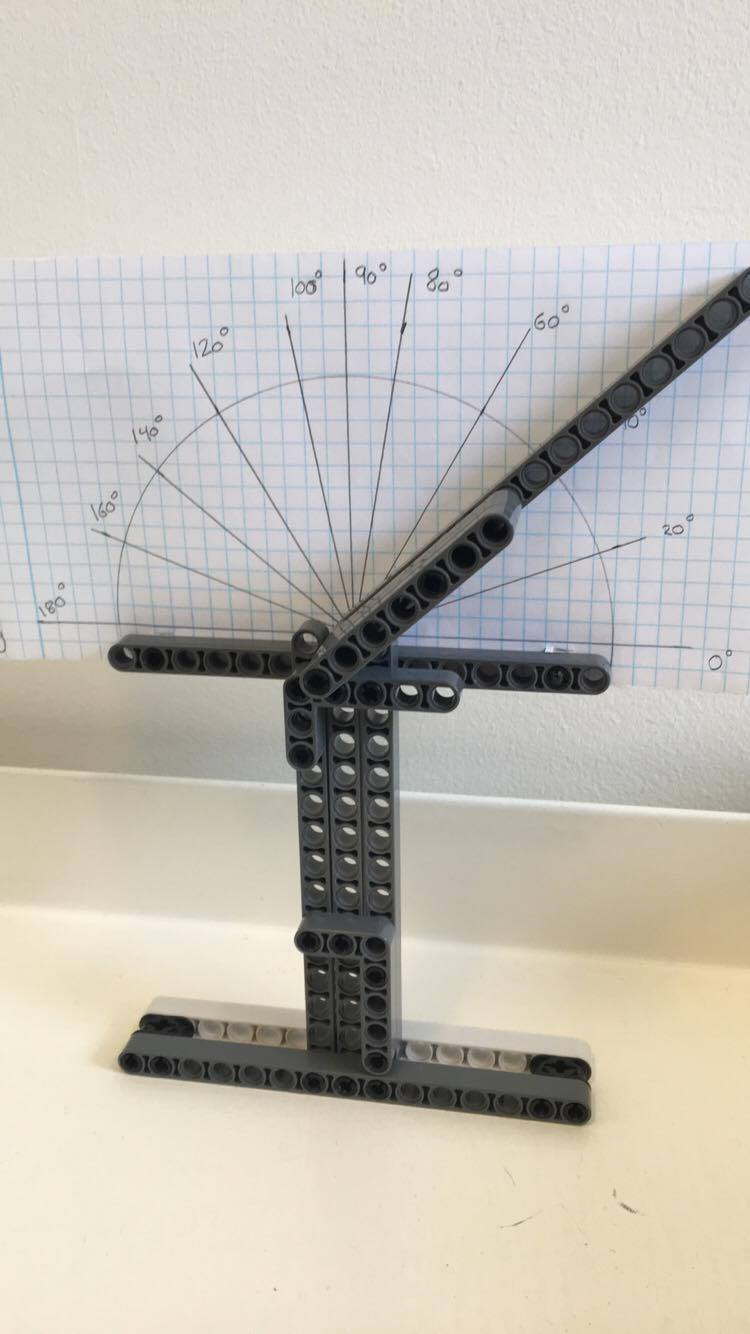
\includegraphics[width=0.3\textwidth]{figures/vinkeltest}
\caption{Vinkeltester, som anvendes under forsøget til at holde accelerometeret i bestemte vinkler}
\label{fig:vinkeltest}
\end{figure}

\subsubsection{Fremgangsmåde for deltest 2}\label{sec:acc_fremgangsmaade}
Der foretages målinger i seks forskellige positioner. Hver position måles tre gange og samles i 10 sekunder ved $100~Hz$. De forskellige positioner er illustreret på \autoref{fig:acc_paavirkning}, og er som følger: 
\begin{itemize}
\item Accelerometeret stilles, så det er lodret opad
\item Accelerometeret stilles, så det er lodret nedad
\item Accelerometeret stilles, så det er vandret mod højre
\item Accelerometeret stilles, så det er vandret mod venstre
\item Accelerometeret ligges plan på bordet opad
\item Accelerometeret ligges plan på bordet nedad
\end{itemize}

\begin{figure}[H]
\centering
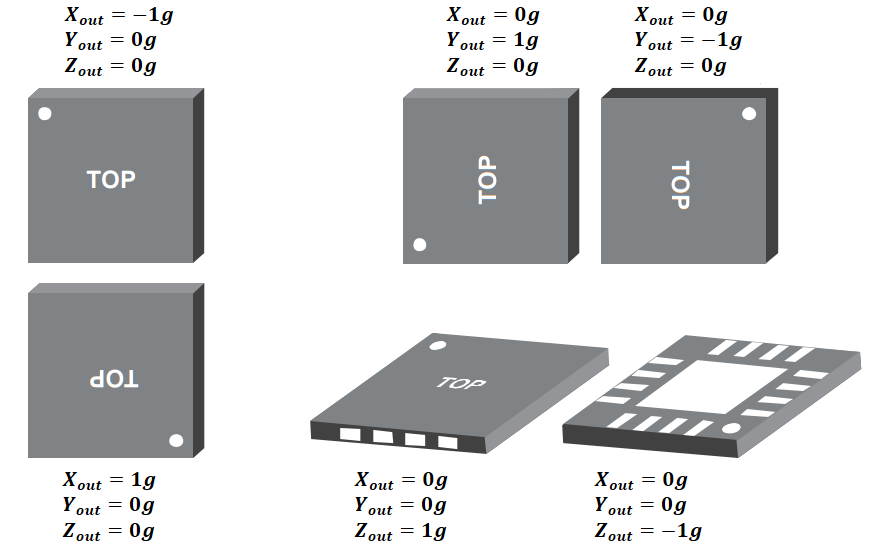
\includegraphics[width=0.5\textwidth]{figures/acc_paavirkning}
\caption{Påvirkning af accelerometeret i forskellige positioner. Til venstre måles accelerometeret i lodret plan, til højre øverst vandret og til højre nederst i plan \citep{analogdevices2010}}
\label{fig:acc_paavirkning}
\end{figure}

\subsection{Resultater} 

\subsubsection{Resultater for deltest 2}

De viste resultater heri er for det ene accelerometer\fxnote{resultaterne er fra det røde accelerometer}, da sensitiviten og offsettet ændrer sig hver gang, der udføres et forsøg. Det vil derfor ikke være muligt at fastsætte konstante værdier for sensitivitet og offset, hvorfor det centrale at udlede er metoden til at beregne værdierne, da udregningerne skal foretages ved hvert forsøg.

Ud fra de tre målinger foretaget i de seks forskellige positioner beregnes den gennemsnitlige værdi af målingerne på de forskellige akser, herefter plottes disse i en graf. På denne måde bliver det muligt at se, hvilken akse der påvirkes mest under øvelsen. Målingerne fremgår af \autoref{fig:acc_paavirkning}. 

\begin{figure}[H]
\centering
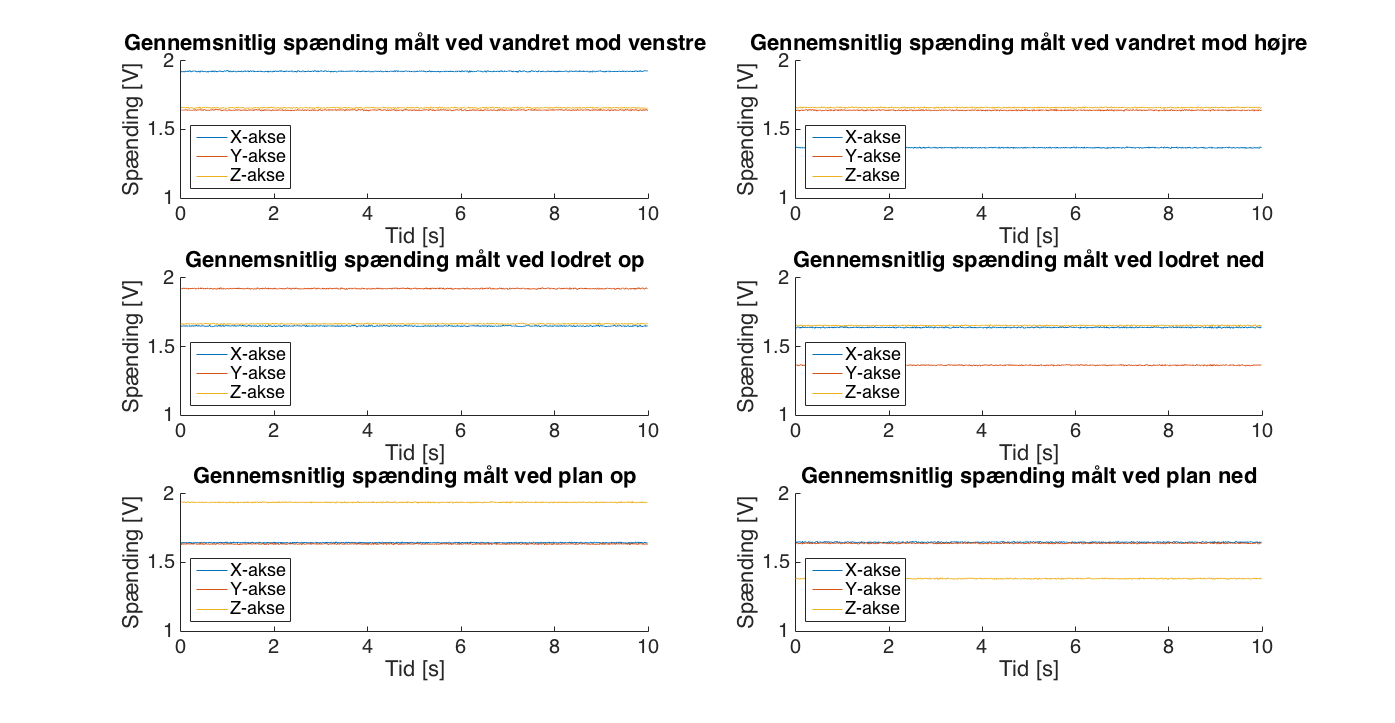
\includegraphics[width=0.8\textwidth]{figures/paavirkning}
\caption{Påvirkningen af accelerometrets tre akser ved de seks forskellige positioner}
\label{fig:acc_paavirkning}
\end{figure}

Offset beregnes ud fra de målinger, hvor accelerometeret påvirkes med 0 g. Den akse hvor accelerometeret påvirkes med 0 g i de seks positioner fremgår af \autoref{fig:acc_paavirkning}. Resultaterne fra målingerne fremgår af \autoref{Tab:acc_offset}. 

\begin{table}[H]
	\centering
	\begin{tabular}{|l|l|l|}
	\textbf{Målt retning} & \textbf{Målt akse} & \textbf{Offset} \\ \hline
    \textbf{Lodret op} 		& X 		& $1,6793~V$ 	\\ \hline
    \textbf{Lodret op} 		& Z 		& $1,6857~V$ 	 \\ \hline
    \textbf{Lodret ned}		& X 		& $1,6750~V$ 	\\ \hline
    \textbf{Lodret ned}		& Z 		& $1,6806~V$  	\\ \hline
    \textbf{Vandret højre} 	& Y 		& $1,6760~V$    \\ \hline     
    \textbf{Vandret højre} 	& Z 		& $1,6828~V$ 	\\ \hline
    \textbf{Vandret venstre}	& Y 		& $1,6755~V$ 	\\ \hline
    \textbf{Vandret venstre}	& Z 		& $1,6836~V$		\\ \hline
    \textbf{Plan op} 		& X 		& $1,6773~V$		\\ \hline		
    \textbf{Plan op} 		& Y 		& $1,6734~V$    \\ \hline
    \textbf{Plan ned} 		& X 		& $1,6787~V$		\\ \hline
    \textbf{Plan ned} 		& Y 		& $1,6755~V$		\\ \hline
	\end{tabular}\label{Tab:acc_offset}
	\caption{Offsettet beregnet for de forskellige akser, hvor accelerometeret udsættes for en 0 g-påvirkning}
\end{table}

Sensitiviten beregnes ud fra forskellen mellem 0 og 1 g-påvirkningen af accelerometeret. Der hvor accelerometeret er påvirket med 1 g er illustreret på \autoref{fig:acc_paavirkning}. Målingerne fremgår af \autoref{Tab:acc_sensitivitet}. 

\begin{table}[H]
	\centering
	\begin{tabular}{|l|l|l|}
	\textbf{Målt retning} & \textbf{Målt akse} & \textbf{Sensitivitet} \\ \hline
    \textbf{Lodret op} 		& Y		& $0,1092~V/g$ 	\\ \hline
    \textbf{Lodret ned}		& Y 		& $-0,1164~V/g$ 	\\ \hline
    \textbf{Vandret højre} 	& X 		& $0,1130~V/g$     \\ \hline     
    \textbf{Vandret venstre}	& X 		& $-0,1167~V/g$ 	\\ \hline
    \textbf{Plan op} 		& Z 		& $0,1232~V/gV$    	\\ \hline		
    \textbf{Plan ned} 		& Z 		& $-0,1079~V/g$		\\ \hline
	\end{tabular}
	\label{Tab:acc_sensitivitet}
	\caption{Sensitiviteten beregnet for de forskellige akser hvor accelerometeret udsættes for en 1 g-påvirkning}
\end{table}

Ud fra senstitivten beregnes spændingen ved $1^{\circ}$ og $90^{\circ}$ i negativ og positiv retning\fxnote{Er der nødvendig med 1 grad?}. Spændingen svarende til $0^{\circ}$ svarer til den målte offsetværdi som fremgår af \autoref{Tab:acc_offset}. Beregningerne af spændingen ved de valgte grader fremgår af \autoref{Tab:acc_grader} og er beregnet ud fra ligning \autoref{equ:vinkler}.

 \begin{table}[H]
	\centering
	\begin{tabular}{|l|l|l|l|}
	\textbf{Målt retning} & \textbf{Målt akse} & \textbf{Spændingen ved grad} & \textbf{Spændingen ved 90 grader} \\ \hline
    \textbf{Positiv} 	& Y		& $1,7985~V$   	&	$12,7589~V$\\ \hline
    \textbf{Negativ}		& Y		& $1,5692~V$  	&	$-8,0339~V$\\ \hline
    \textbf{Positiv} 	& X 		& $1,7917~V$   	& 	$11,5105~V$ \\ \hline     
    \textbf{Negativ}		& X 		& $1,5614~V$		&	$-8,7982~V$\\ \hline
    \textbf{Positiv} 	& Z 		& $1,7924~V$   	& 	$11,8494~V$	\\ \hline		
    \textbf{Negativ} 	& Z 		& $1,5629~V$		&	$-8,8190~V$ \\ \hline
	\end{tabular}
	\caption{Beregnet spænding ved henholdsvis 1 og 90 grader i positiv og negativ retning}
	\label{Tab:acc_grader}
\end{table}







%\fi
\end{document}
